\documentclass[autodetect-engine,12pt,titlepagedvi=dvipdfmx,ja=standard]{bxjsreport} 
%\documentclass[a4paper,12pt]{bxjsreport}
%\documentclass[a4paper,12pt,titlepage]{jsreport}
%\documentclass[autodetect-engine,12pt,titlepagedvi=dvipdfmx,ja=standard,twocolumn,jbase=13.35Q]{bxjsarticle} 
%jbase=13.35Qは和文フォントサイズを9.5ptにする指定です。おおよそ和文フォントの単位(Q:級)では、13.35Q=9.5ptです。

\usepackage{bm}
\usepackage[dvipdfmx]{graphicx}
\usepackage{ascmac}
\usepackage{url}

\usepackage{amsmath, amssymb}

\usepackage[subrefformat=parens]{subcaption}
\usepackage{pdfpages}

\usepackage{comment}

\usepackage{graphicx}
\usepackage{color}

%%% ヘッダに章とページ番号を記載
\pagestyle{headings}

\title{卒業論文\\頭部伝達関数の機械学習に基づく\\
前後方向の音像識別に関する検討}
\author{岩手大学理工学部システム創成工学科\\
知能・メディア情報コース\\永田研究室\\S0617034 瀬音光一}

\date{}

\begin{document}

%%%% タイトル
\maketitle
%%%% 目次
\tableofcontents

%%%%% はじめに
\chapter{はじめに}

前後方向の音像の識別には、頭の形、特に耳介の形
と前後の非対称性が大きく影響していることが知られている。
この非対称により、同一の信号音でも前方から来た場合と後方から来た場合とでは、
各々の周波数特性が異なる。
この周波数特性上の方向定位に関する手掛かりをスペクトルキューと呼び、
前後方向のスペクトルキューについては、頭部伝達関数(HRTF:Head-Related Transfer Fuction)
の4kHz付近に存在するピーク(P1)、及び4kHz以上に存在する最初のノッチ(N1)とその次の
ノッチ(N2)が知られているが\cite{K}、
HRTFは音源の信号が既知でないと推定できないはずであり、
またスペクトル上のノッチは背景雑音によって容易に消失してしまうため、
ヒトがノイズの存在する環境の中でその差異をどのように識別し、学習しているかは明らかではない。
%HRTFではなく両耳間レベル差(ILD:Interaural Level Difference)
そこで、本研究では
%実世界においては従来のHRTFではなく、両耳間の相関によってヒトは前後の識別を学習していると考え、
特に音像制御の難度が高いとされている前後の定位\cite{K2}について
機械学習を用いてその学習が可能であるかを検討する。

\section{検証実験}
機械学習を用いての実験の前に、実際に前後の判別を行えるか20代男女(計2名)で検証を行った。
検証方法は、無教室内で前後1mにスピカーを設置し、ランダムにどちらか一方向から音源を流すという方法で行った。
使用した音源は、音声、効果音、音楽(ボーカル有り)を各々10データ、各音源の時間長は3秒弱であり、
試行回数は、両耳、左耳のみ、右耳のみを各々30データ分行った。
その結果、両耳では30問全て正解したのに対し、片耳では30問中1〜2問不正解があった。
また、不正解に関しては、一人は右耳で、もう一方は左耳で発生した。
これは、頭部伝達関数の個人差によるものであると考えられる。
試験者の感想としては、「片耳の場合に前後どちらか分からない事があった」と本人たちも自覚している。
このことからも、先述した頭部伝達関数だけでは前後の学習は不十分であると考える。


\section{本研究の流れ}
本研究の処理の流れを図\ref{fig:1_1}に示し、以下の手順で進めていく。
図中の$_l,_r$は、左右の耳を表す。

①,音源信号の準備

②,①で準備した音源信号とダミーヘッドを用いて録音信号を録音する。

③,②で録音した録音信号に、別途録音したノイズ信号をSN比10dBになるように\\    加え雑音重畳録音信号を求める。

④,③で求めた雑音重畳録音信号からHRTFとILDを求める。

⑤,機械学習により④で求めたHRTFとILDの識別率を各々求め、比較する。


\begin{figure}[htbp]
  \begin{center}
  \includegraphics[clip, width=5.0in, height = 2.5in]{picture/ProcessFlowOfThisResearch.png}
  \end{center}
  \caption{本研究の処理の流れ}\label{fig:1_1}
\end{figure}

\chapter{断片的な信号音による到来方向識別}
音響伝達関数推定に使われる掃引正弦波や白色雑音といった人工的な信号を方向識別の学習信号として用いれば、
%精度の高いHRTFが推定可能であり、これを用いれば
前後の識別は比較的容易であると考えられるが、ヒトは測定用信号ではなく、
時間的にも周波数の上でも断片的で片寄った信号から到来方向に関する学習を行っているものと考えられる。
また先述したように、
HRTFは音源の信号が既知でないと推定できないはずであり、
背景雑音が伝達関数上のノッチを隠し、さらに学習の精度を低下させるものと考えられる。

そこで、本研究では伝達関数測定用の人工的な信号ではなく、
実世界で到来するような断片的な信号から不完全な前後のHRTFと両耳間レベル差(ILD:Interaural Level Difference)の集合を求め、
これらを入力とした機械学習による前後の識別について検討する。
%前後の識別がそれらの機械学習によって可能か各々検討する。\\
    
\section{録音方法}
使用した音源は、音声、効果音、ボーカル入り音楽の3種類で時間長は各々3秒弱である。
%音源の内訳は、音声72、効果音60、音楽88、合計220であり、
音源の内訳は表\ref{tb:fugafuga1}に示したとおりであり、各々3秒ごとに録音を行った。
録音はダミーヘッドの両耳にマイクロホンを装着し、図\ref{fig:0}に示す環境で行った。
また、録音信号には別途ダミーヘッドで録音した左右の背景雑音をSN比10dBとなるように加えた。

\begin{table}[htbp]
  \centering
  \begin{tabular}{l|c}
    分類 & 時間長(s)  \\ \hline\hline
    音声 & 216  \\
    効果音 & 180  \\
    音楽(ボーカル有り) & 264  \\ \hline
    合計 & 660  \\
  \end{tabular}
  \caption{音源の分類}
  \label{tb:fugafuga1}
\end{table}

\begin{figure}[htbp]
\begin{center}
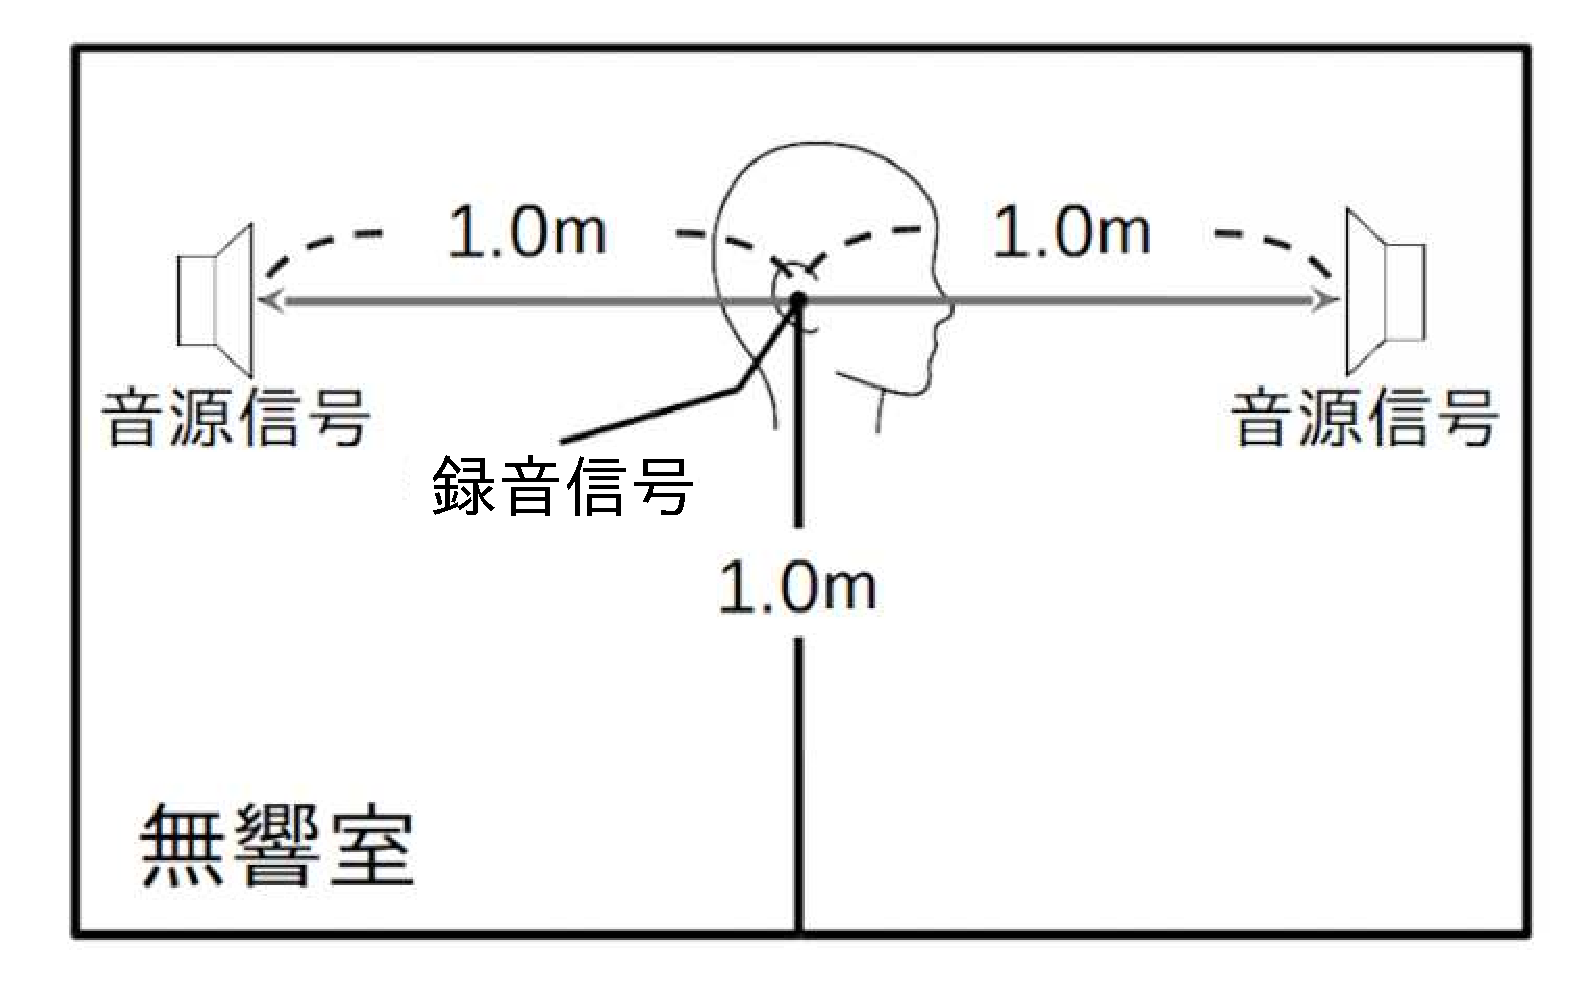
\includegraphics[clip, width=3.0in, height = 2.0in]{picture/environment.eps}
\end{center}
\caption{録音環境}\label{fig:0}
\end{figure}

\clearpage

\section{前後の頭部伝達関数の測定}
HRTF推定
は$X$と$Y_l,_r$とのクロススペクトル法により算出した。
計算式を式\ref{formula:HRTF}に示す。
ここで、添字の$_l,_r$は各々左右の耳を表し、$X$と$Y$は各々
音源信号及び、背景雑音を加えた録音信号に対し
1024点のDFTスペクトル
により得られた512点の複素数から
クロススペクトル法によりHRTFを算出した。

%\\$HRTFl,r(w) = El,r(w)/ F(w) (1)$\\
\begin{equation}
     %&HRTFl,r(w) = El,r(w)/ F(w)
     HRTF_l,_r(k) = \frac{\overline{ Y_l,_r(k)*X(k)^{*} }}{ \overline{ X(k)*X(k)^{*} }}\label{formula:HRTF}
\end{equation}

  %$Asignal$\\
  %$Anoise$\\

  %上記の環境で、
  上記で白色雑音と220の信号からHRTFを求めた。
  白色雑音のHRTFを図\ref{fig:whitenoiseHRTF}に、
  220の信号ごとに得られたHRTFのうち例として3つを図\ref{fig:HRTF}に示す。
  図\ref{fig:whitenoiseHRTF}と図\ref{fig:HRTF}を比べると、
  %&白色雑音では、6kHz付近のノッチで前後の判断が可能であり先行研究\cite{K}と一致する結果が得られた。
  白色雑音では、音源が前方の場合は6kHz付近にノッチが存在し、音源が後方の場合には10kHz付近にノッチが確認でき、
  前後の判断が目視でも可能であり、先行研究\cite{K}と一致する結果が得られた。 
  一方、雑音重畳両耳録音信号でも前後のノッチが異なる位置に確認できたが、白色雑音と比べるとその違いが弱くなっており
  目視だけでは前後の判別が困難であっり、これは雑音による影響であると考える。
  
  %前後の特徴を見出すことが困難であった。
  
  \begin{comment}
    一方、図\ref{fig:A}から分かるように、実音源による伝達関数は雑音ののような振幅のばらつきがあり、
    そのままでは差異の確認が難しいため、
    目視でも差異を確認できるようにスムージングを行った。その結果を図\ref{fig:B}に示す。
    その結果、図\ref{fig:B}の四角部分に違いを確認できる。
    スムージングには、Savizky-Golay法を使用した。
特徴が見られる8kHz~15kHz区間だけ出力したものが図\ref{fig:C}になる。
この区間で機械学習による識別を行うことにした。
\end{comment}

\clearpage

%HRTF
\begin{figure}[htbp]
  \begin{tabular}{cc}
    \begin{minipage}[t]{0.45\hsize}
      \centering
      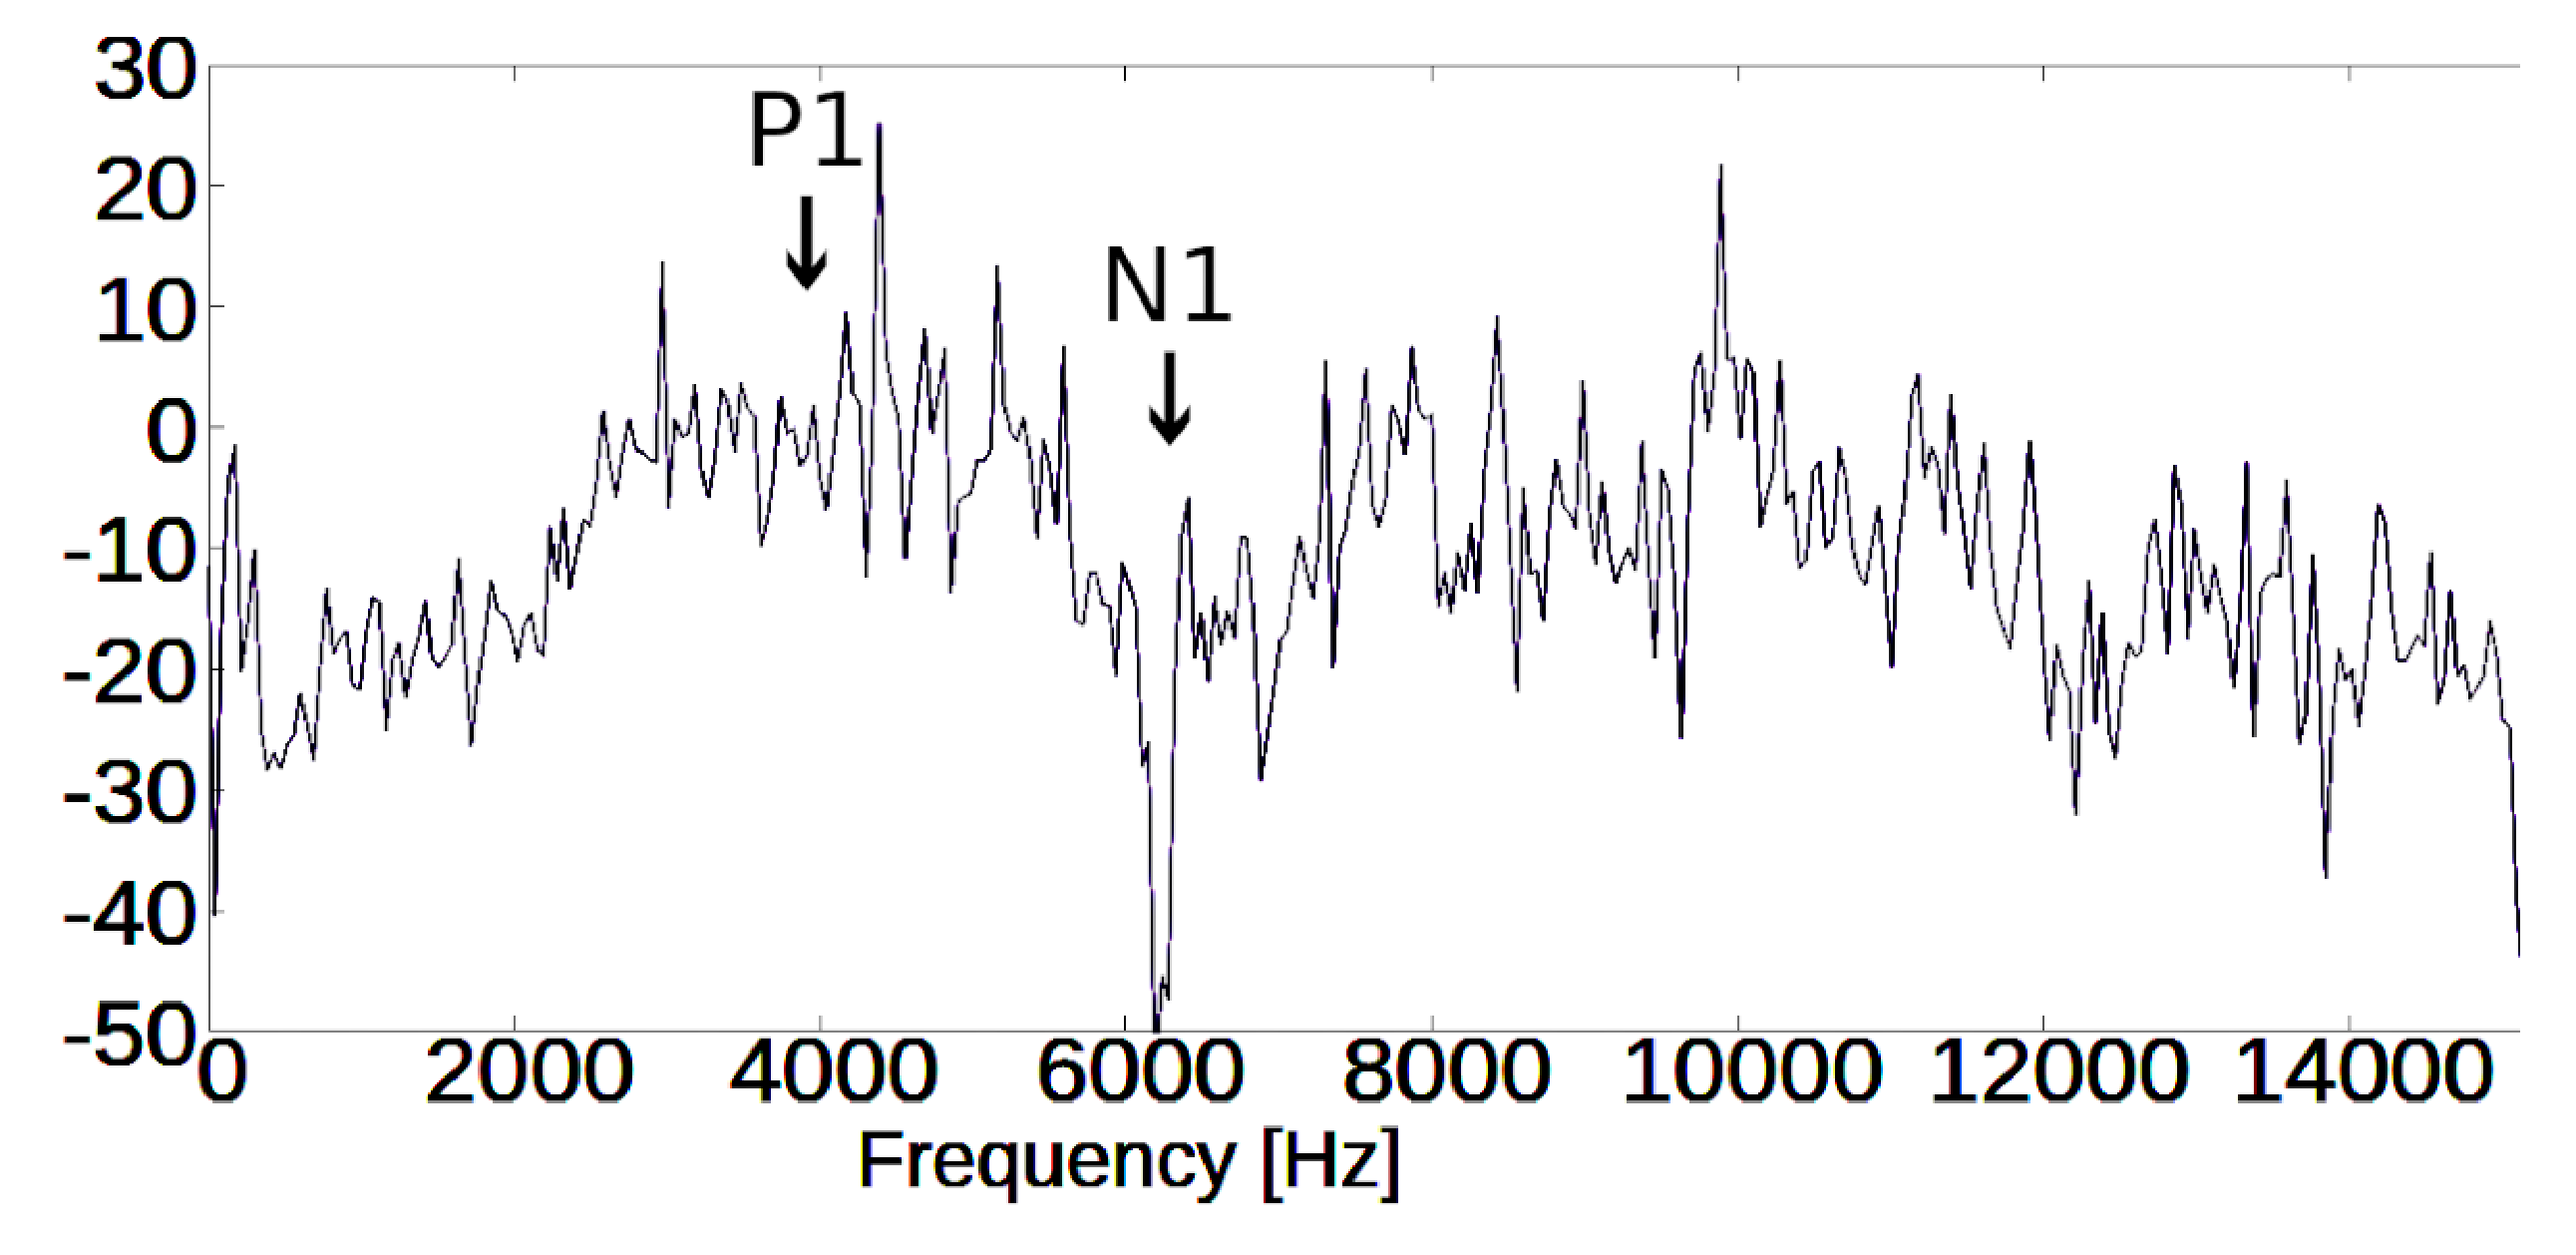
\includegraphics[keepaspectratio, scale=0.14]{picture/wn_mae_l.eps}
      \subcaption{音源が前方で左耳の場合}
     
    \end{minipage} &
    \begin{minipage}[t]{0.45\hsize}
      \centering
      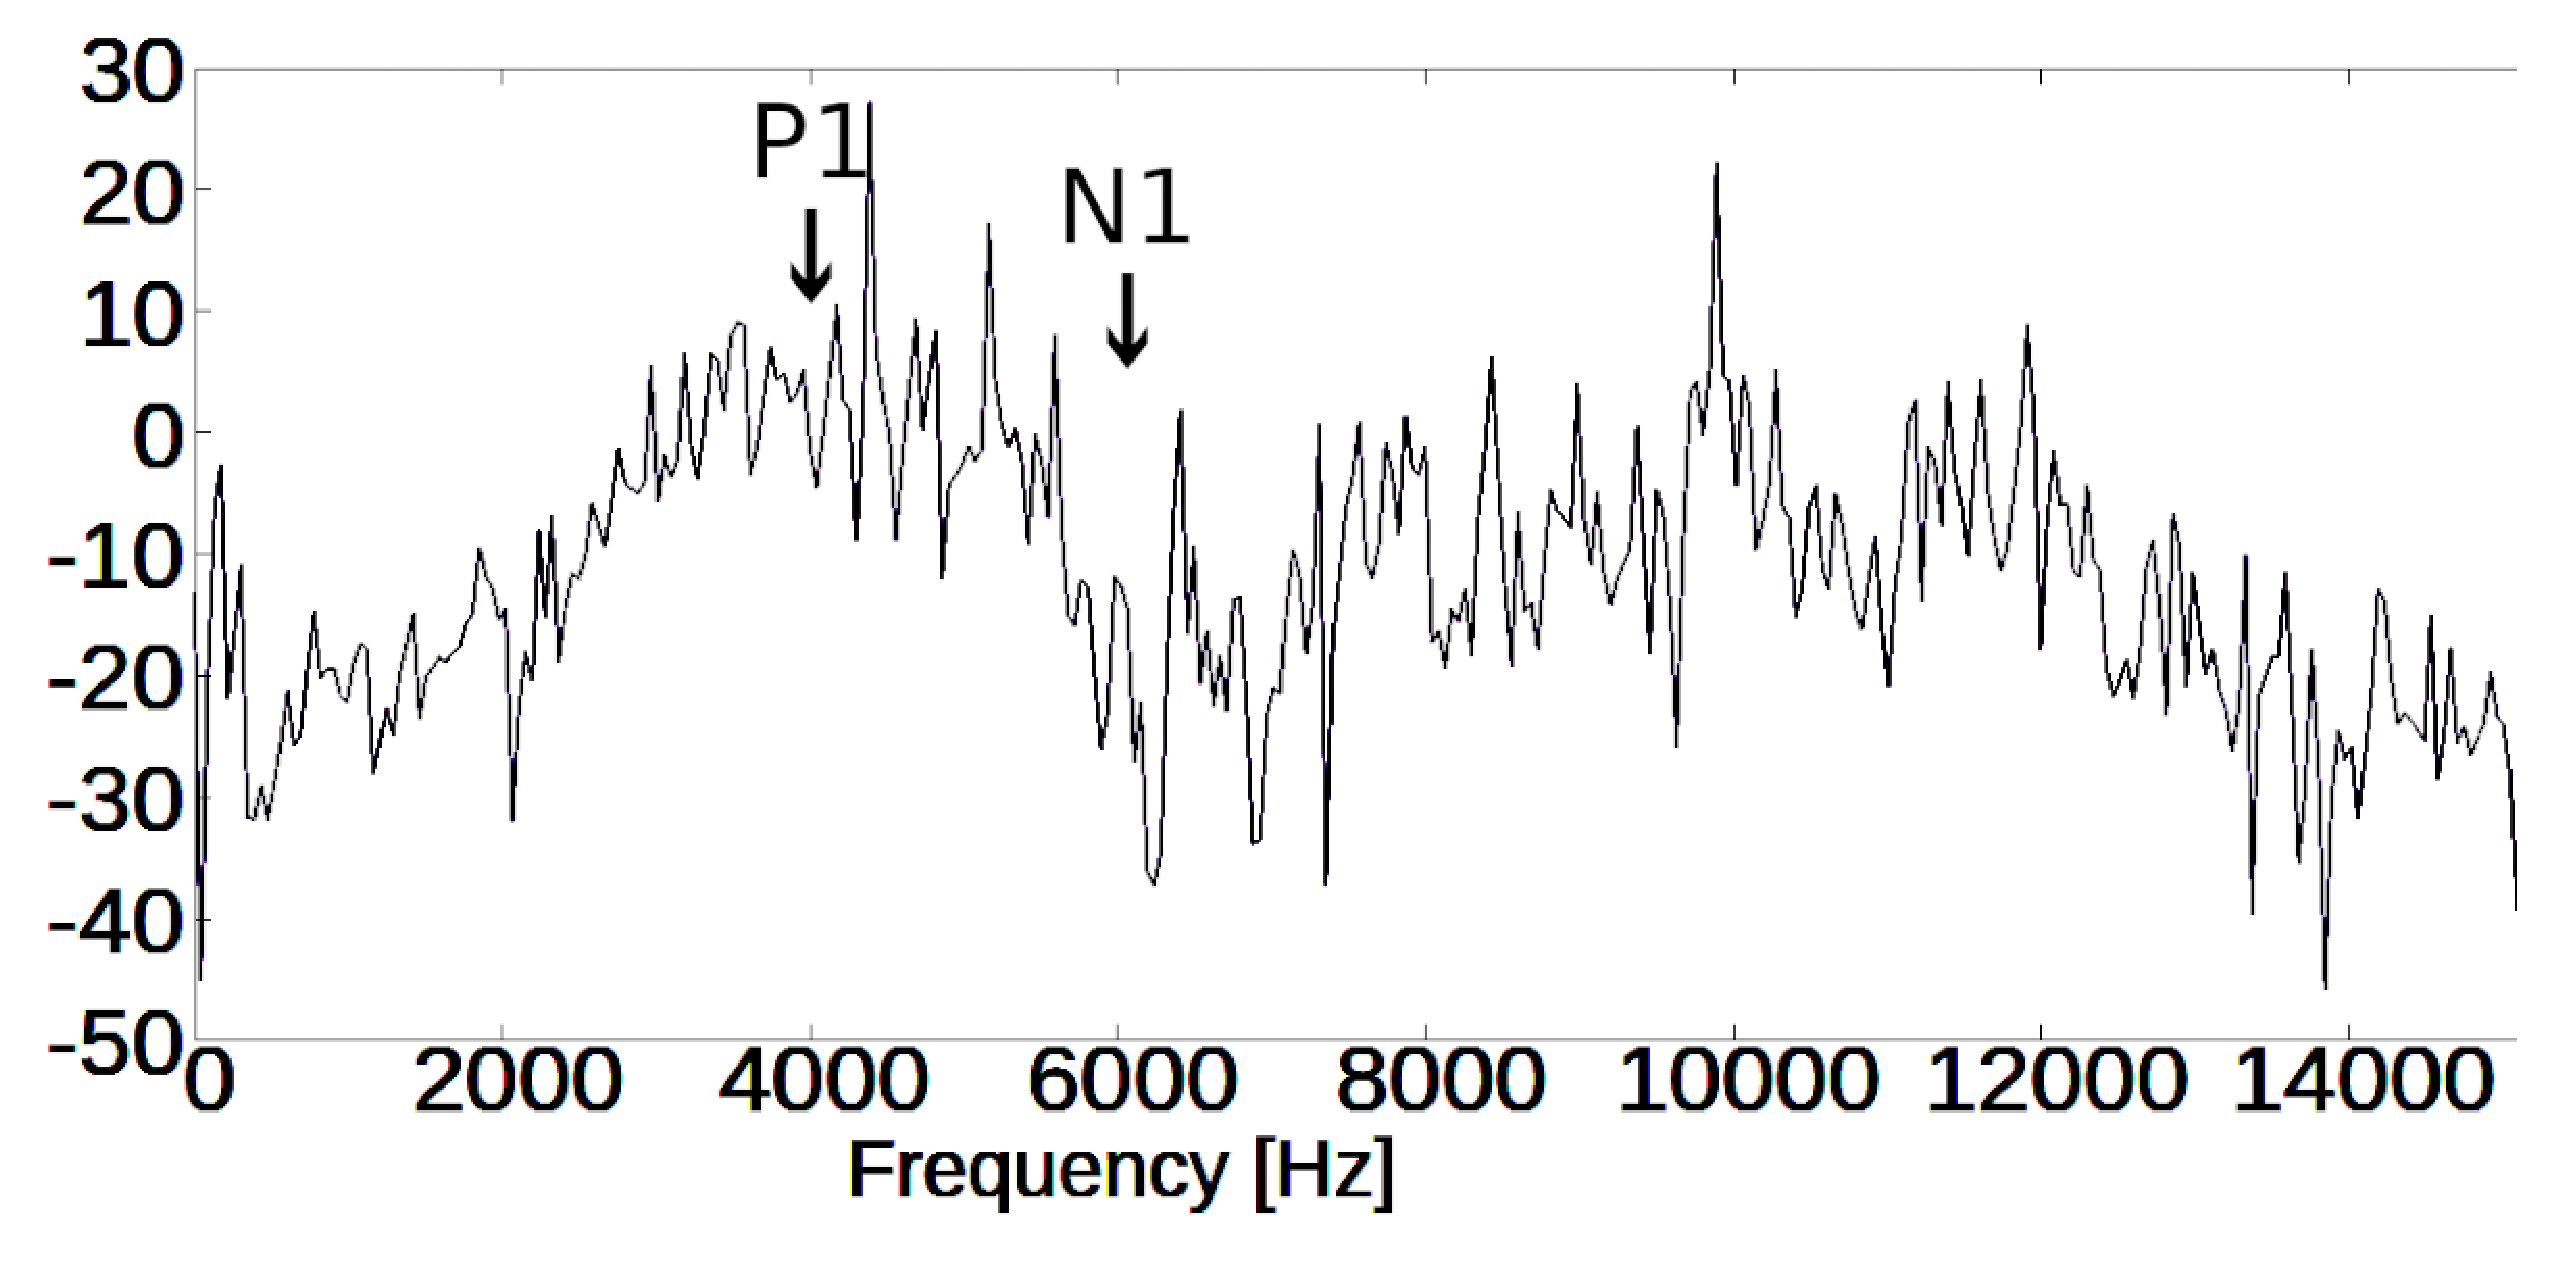
\includegraphics[keepaspectratio, scale=0.14]{picture/wn_mae_r.eps}
      \subcaption{音源が前方で右耳の場合}

    \end{minipage} \\
 
    \begin{minipage}[t]{0.45\hsize}
      \centering
      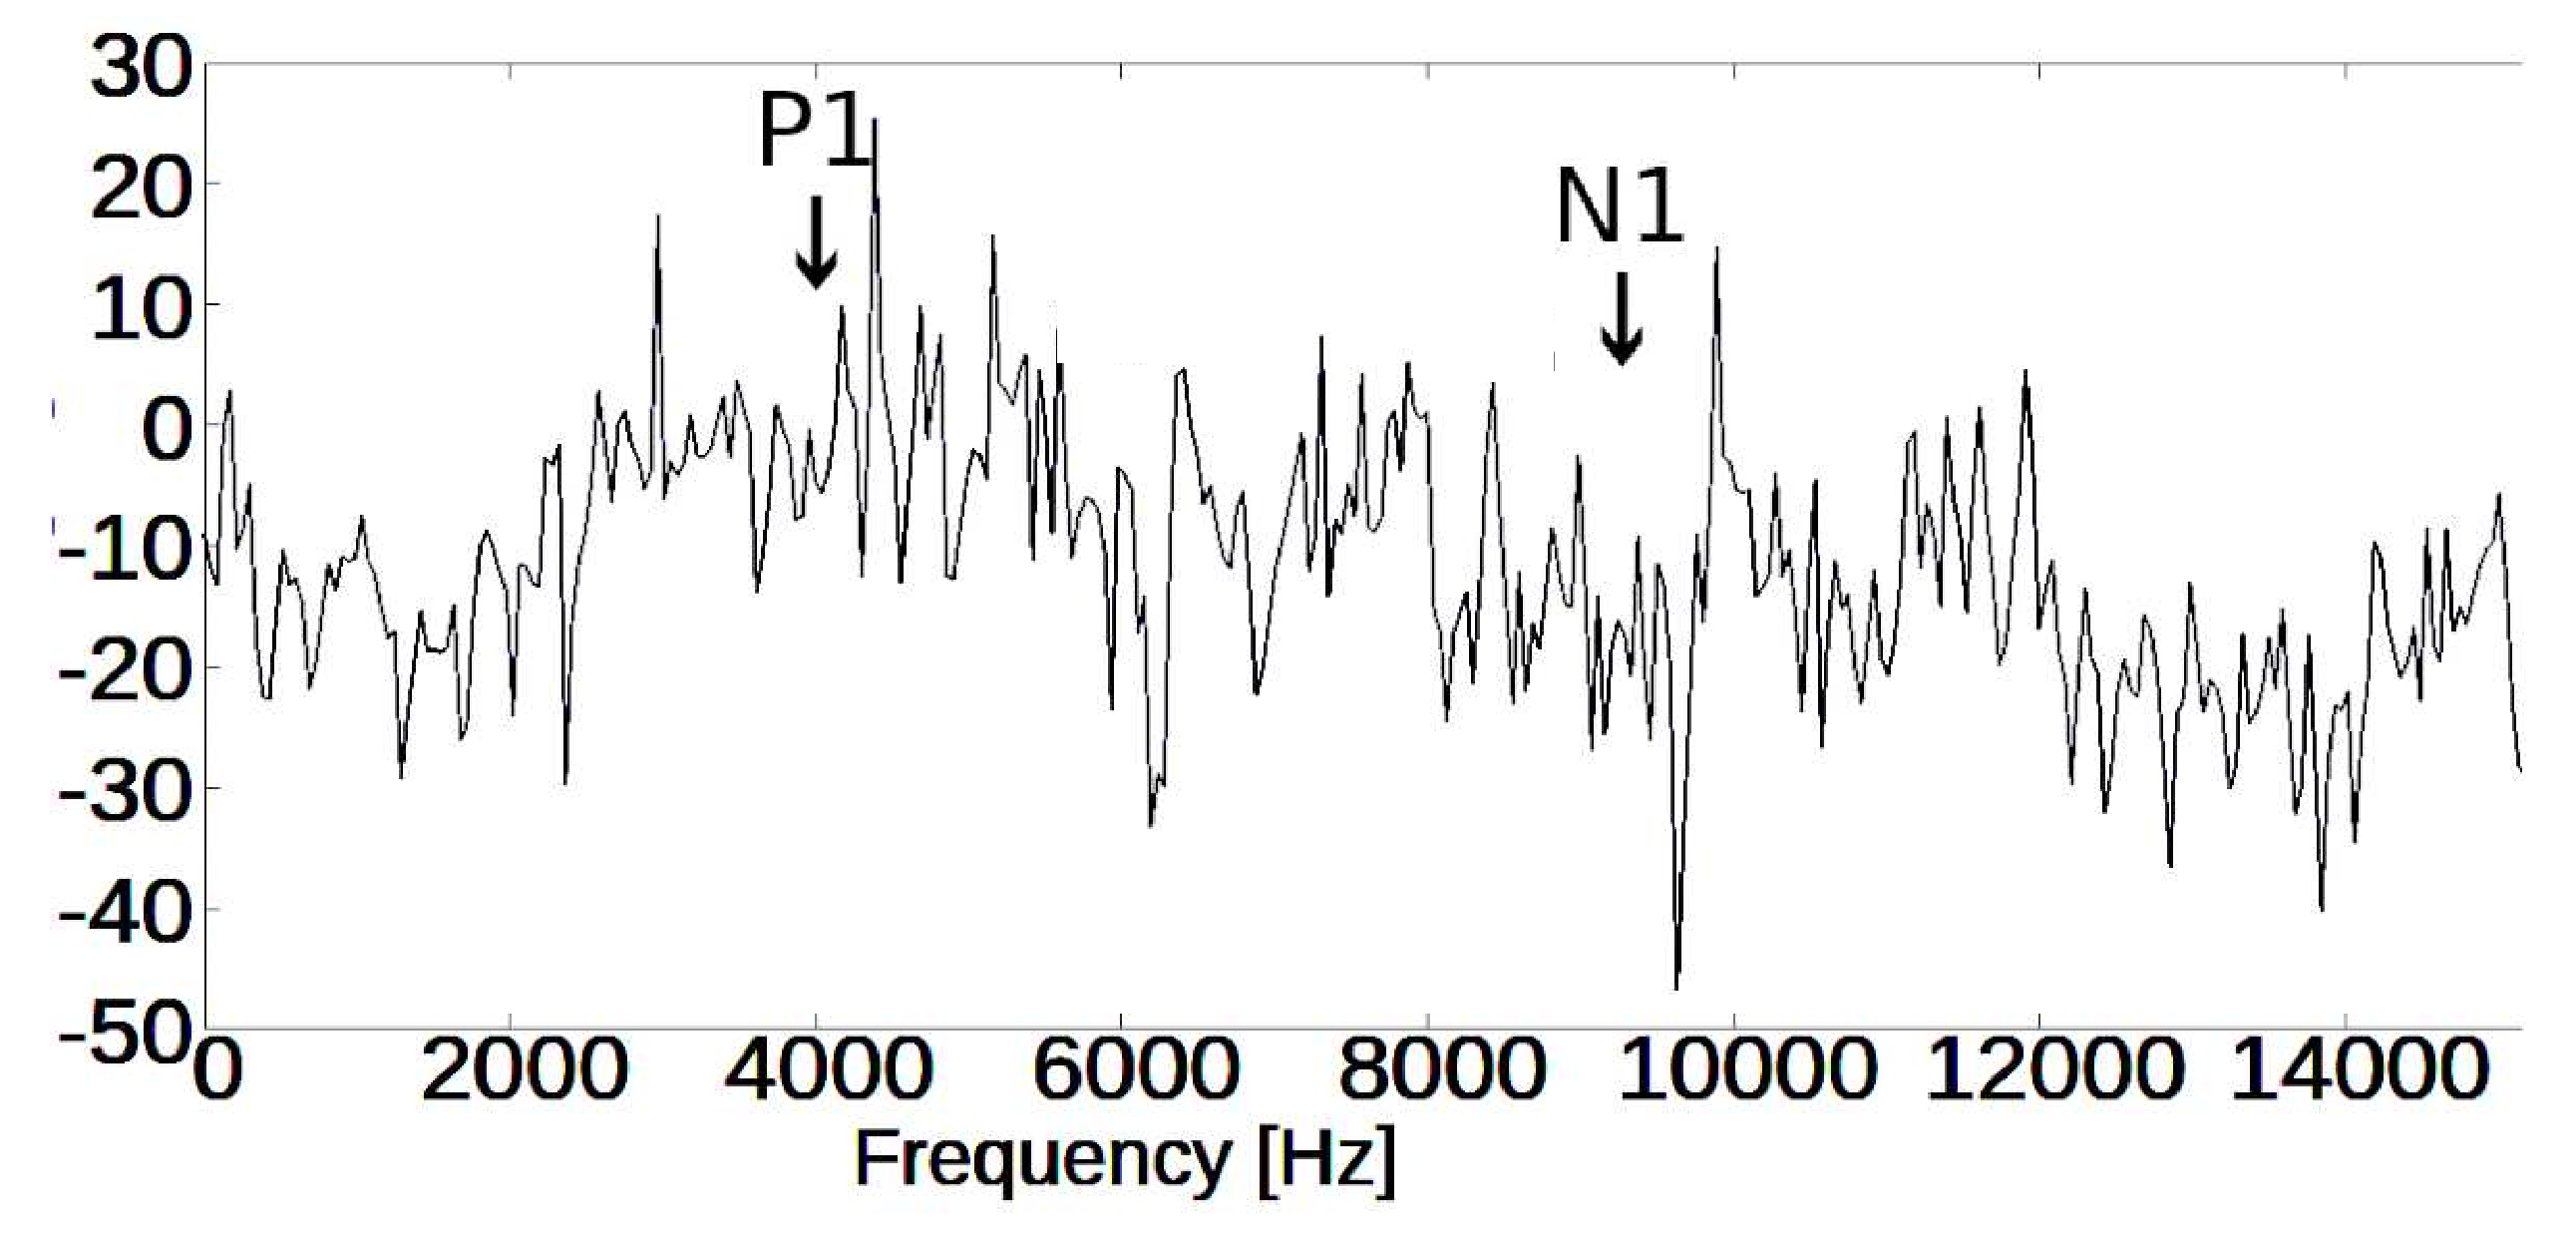
\includegraphics[keepaspectratio, scale=0.14]{picture/wn_usiro_l.eps}
      \subcaption{音源が後方で左耳の場合}

    \end{minipage} &
    \begin{minipage}[t]{0.45\hsize}
      \centering
      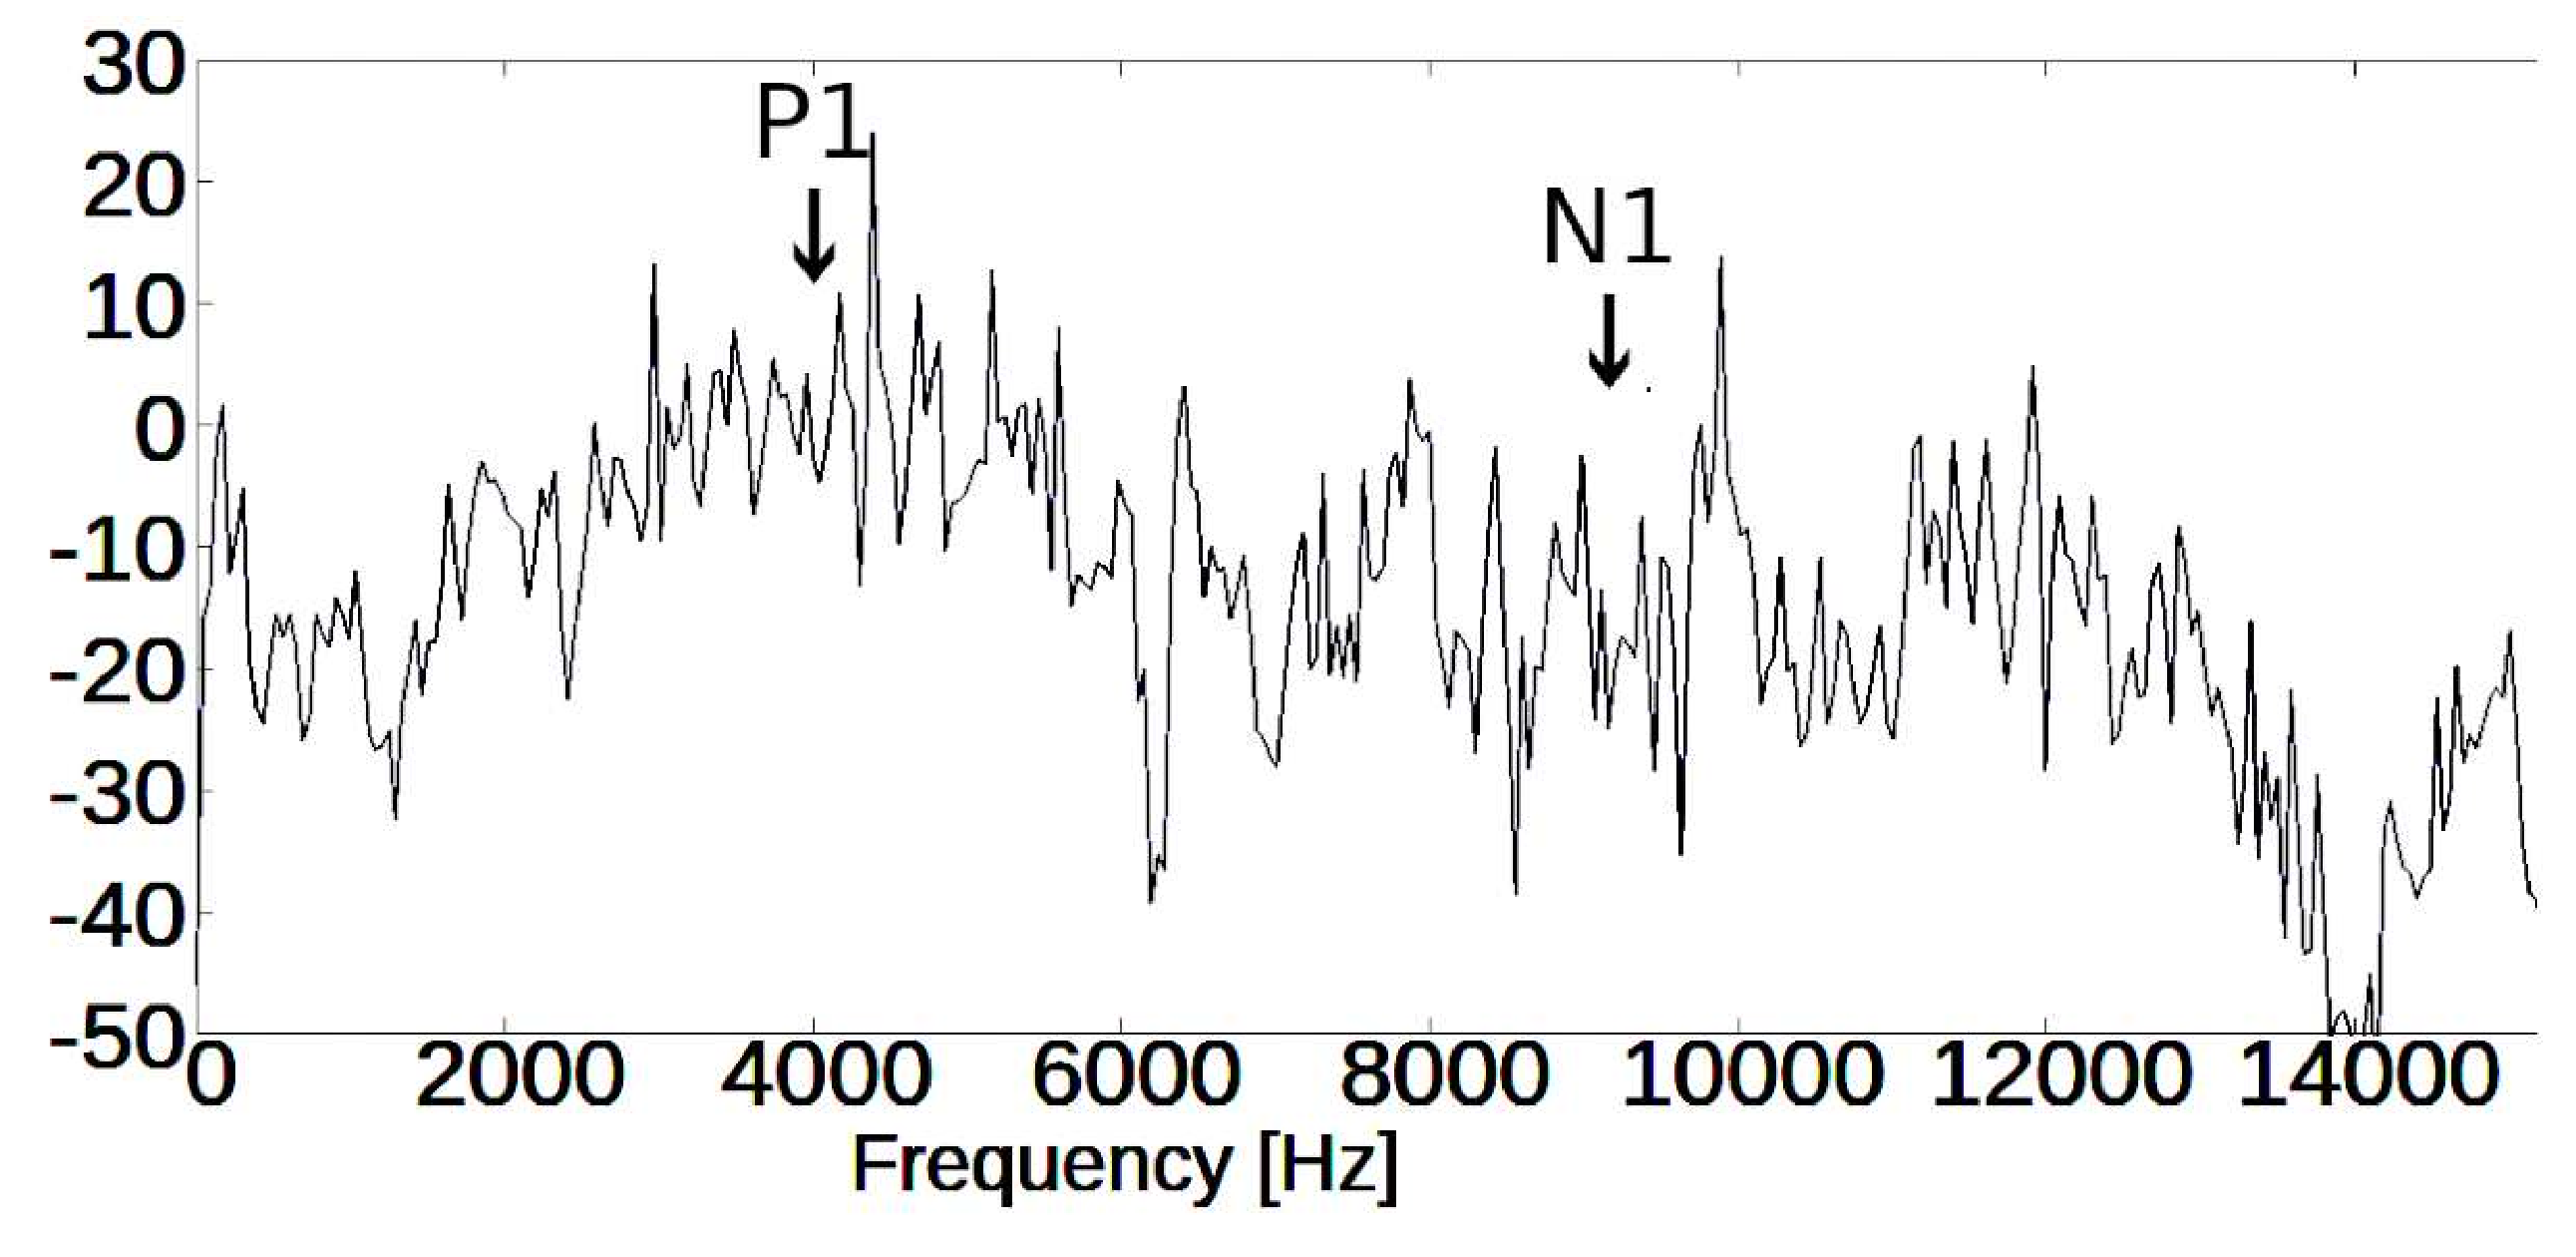
\includegraphics[keepaspectratio, scale=0.14]{picture/wn_usiro_r.eps}
      \subcaption{音源が後方で右耳の場合}

    \end{minipage}
  \end{tabular}
   \caption{白色雑音を用いて測定した頭部伝達関数}\label{fig:whitenoiseHRTF}
%\end{figure}
%\begin{figure}[htbp]
  \begin{tabular}{cc}
    \begin{minipage}[t]{0.45\hsize}
      \centering
      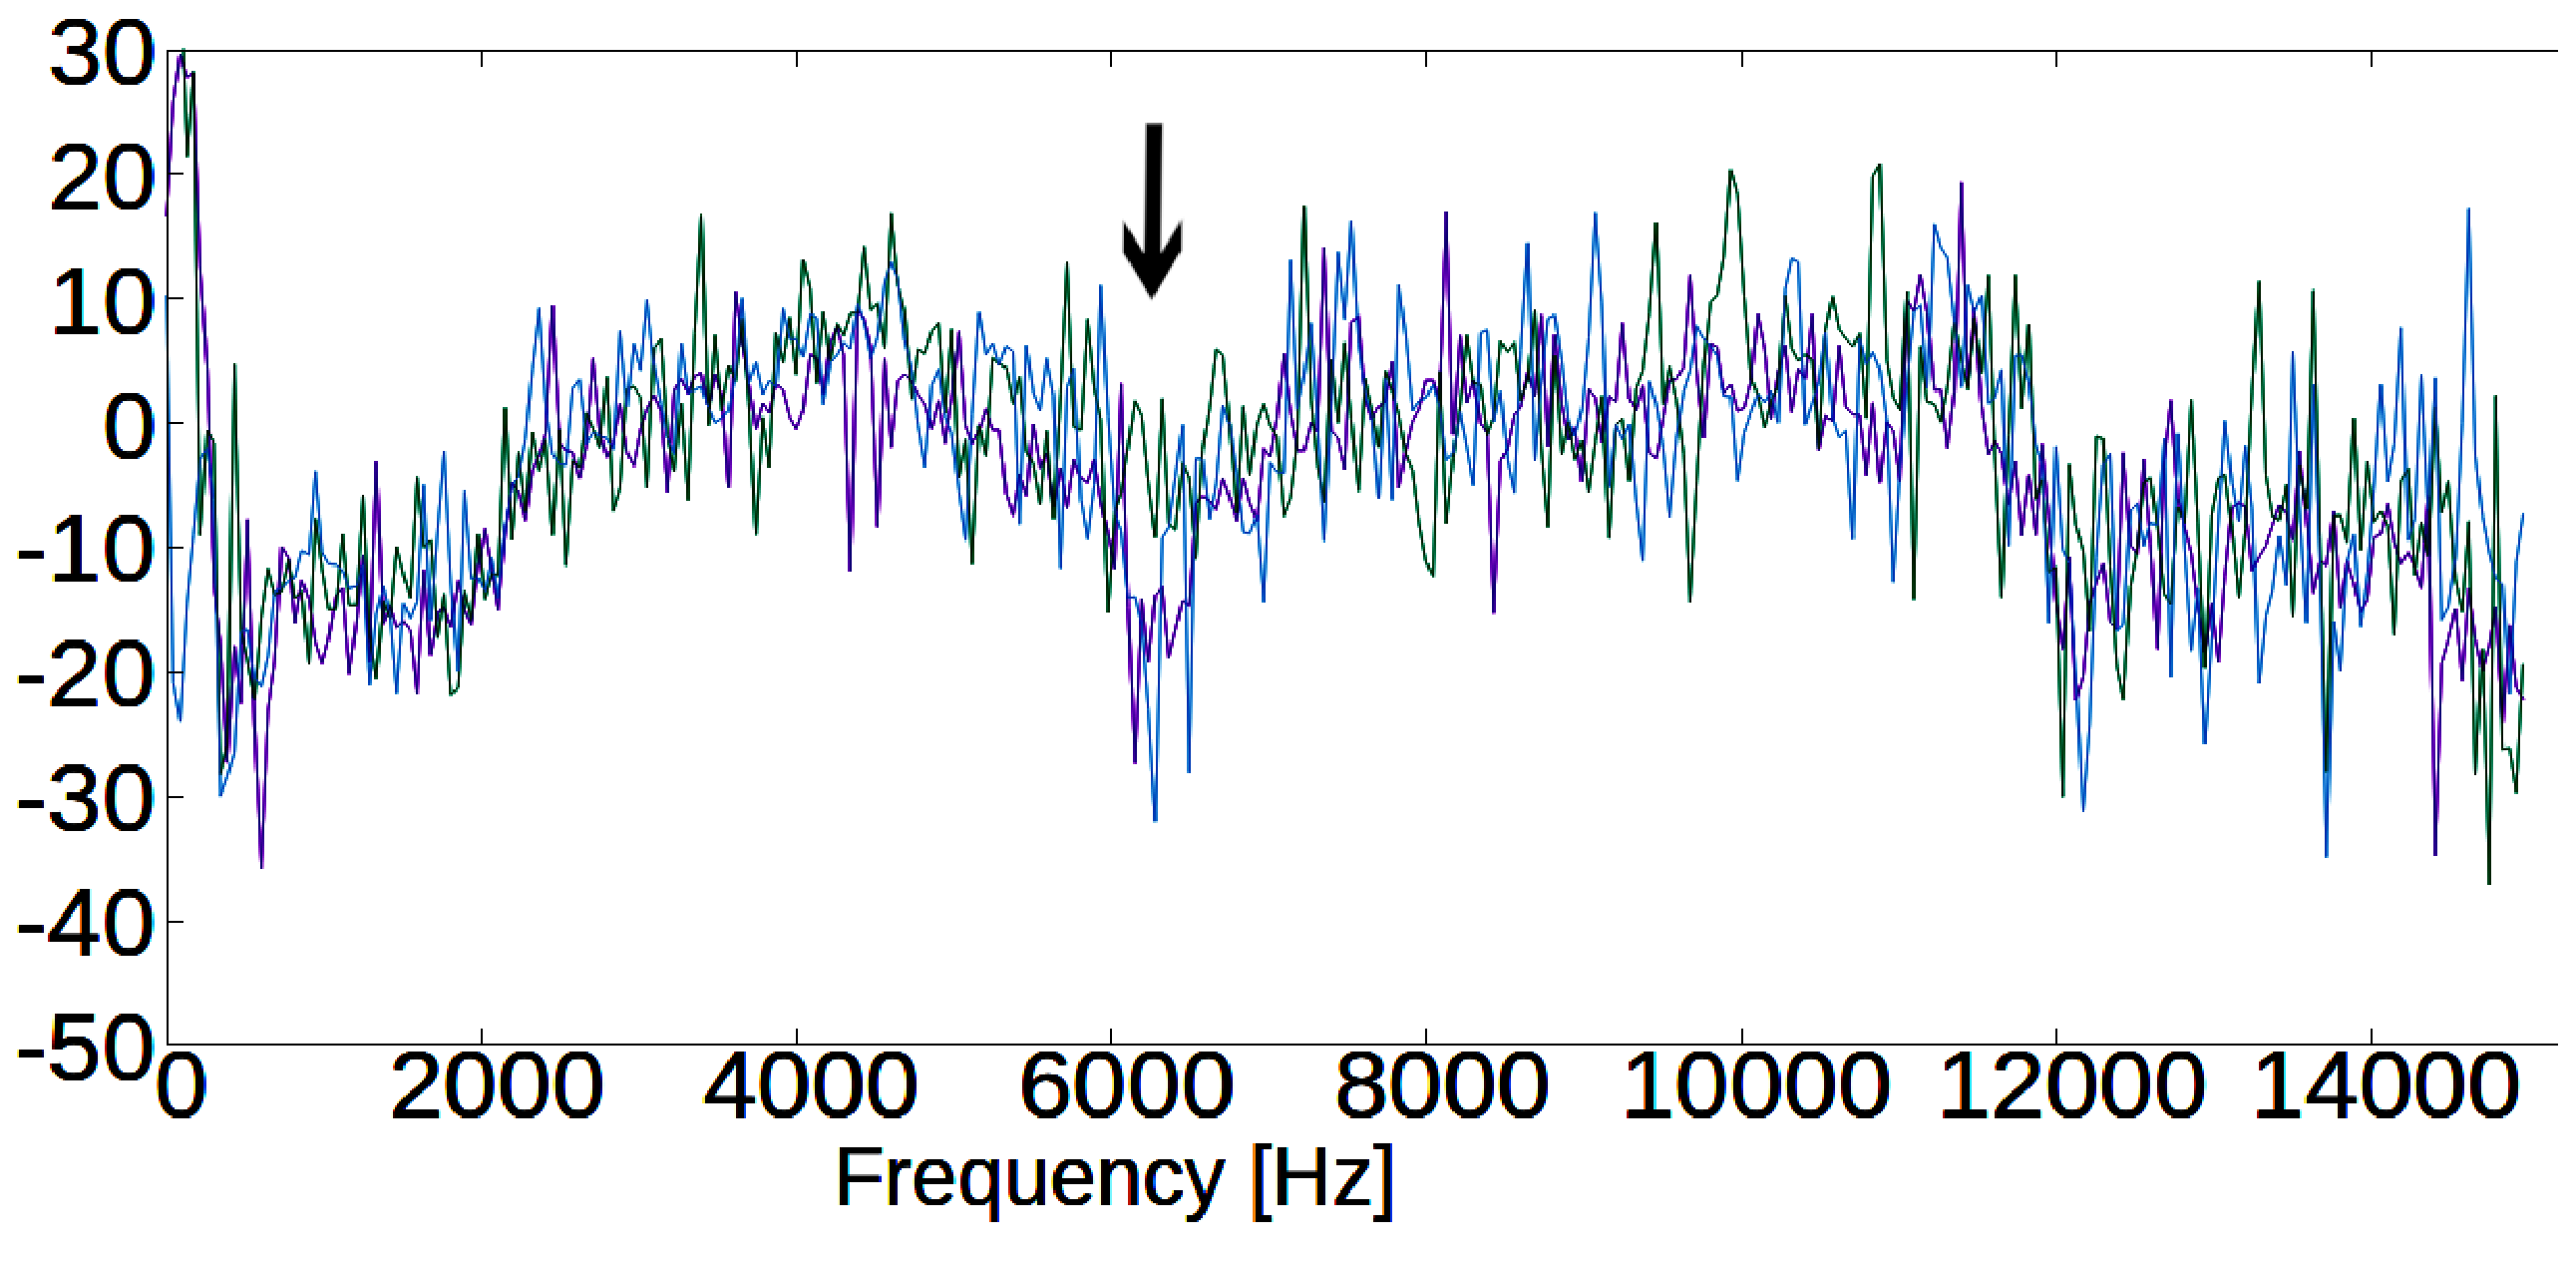
\includegraphics[keepaspectratio, scale=0.14]{picture/No1-3_mae_l.eps}
      \subcaption{音源が前方で左耳の場合}

    \end{minipage} &
    \begin{minipage}[t]{0.45\hsize}
      \centering
      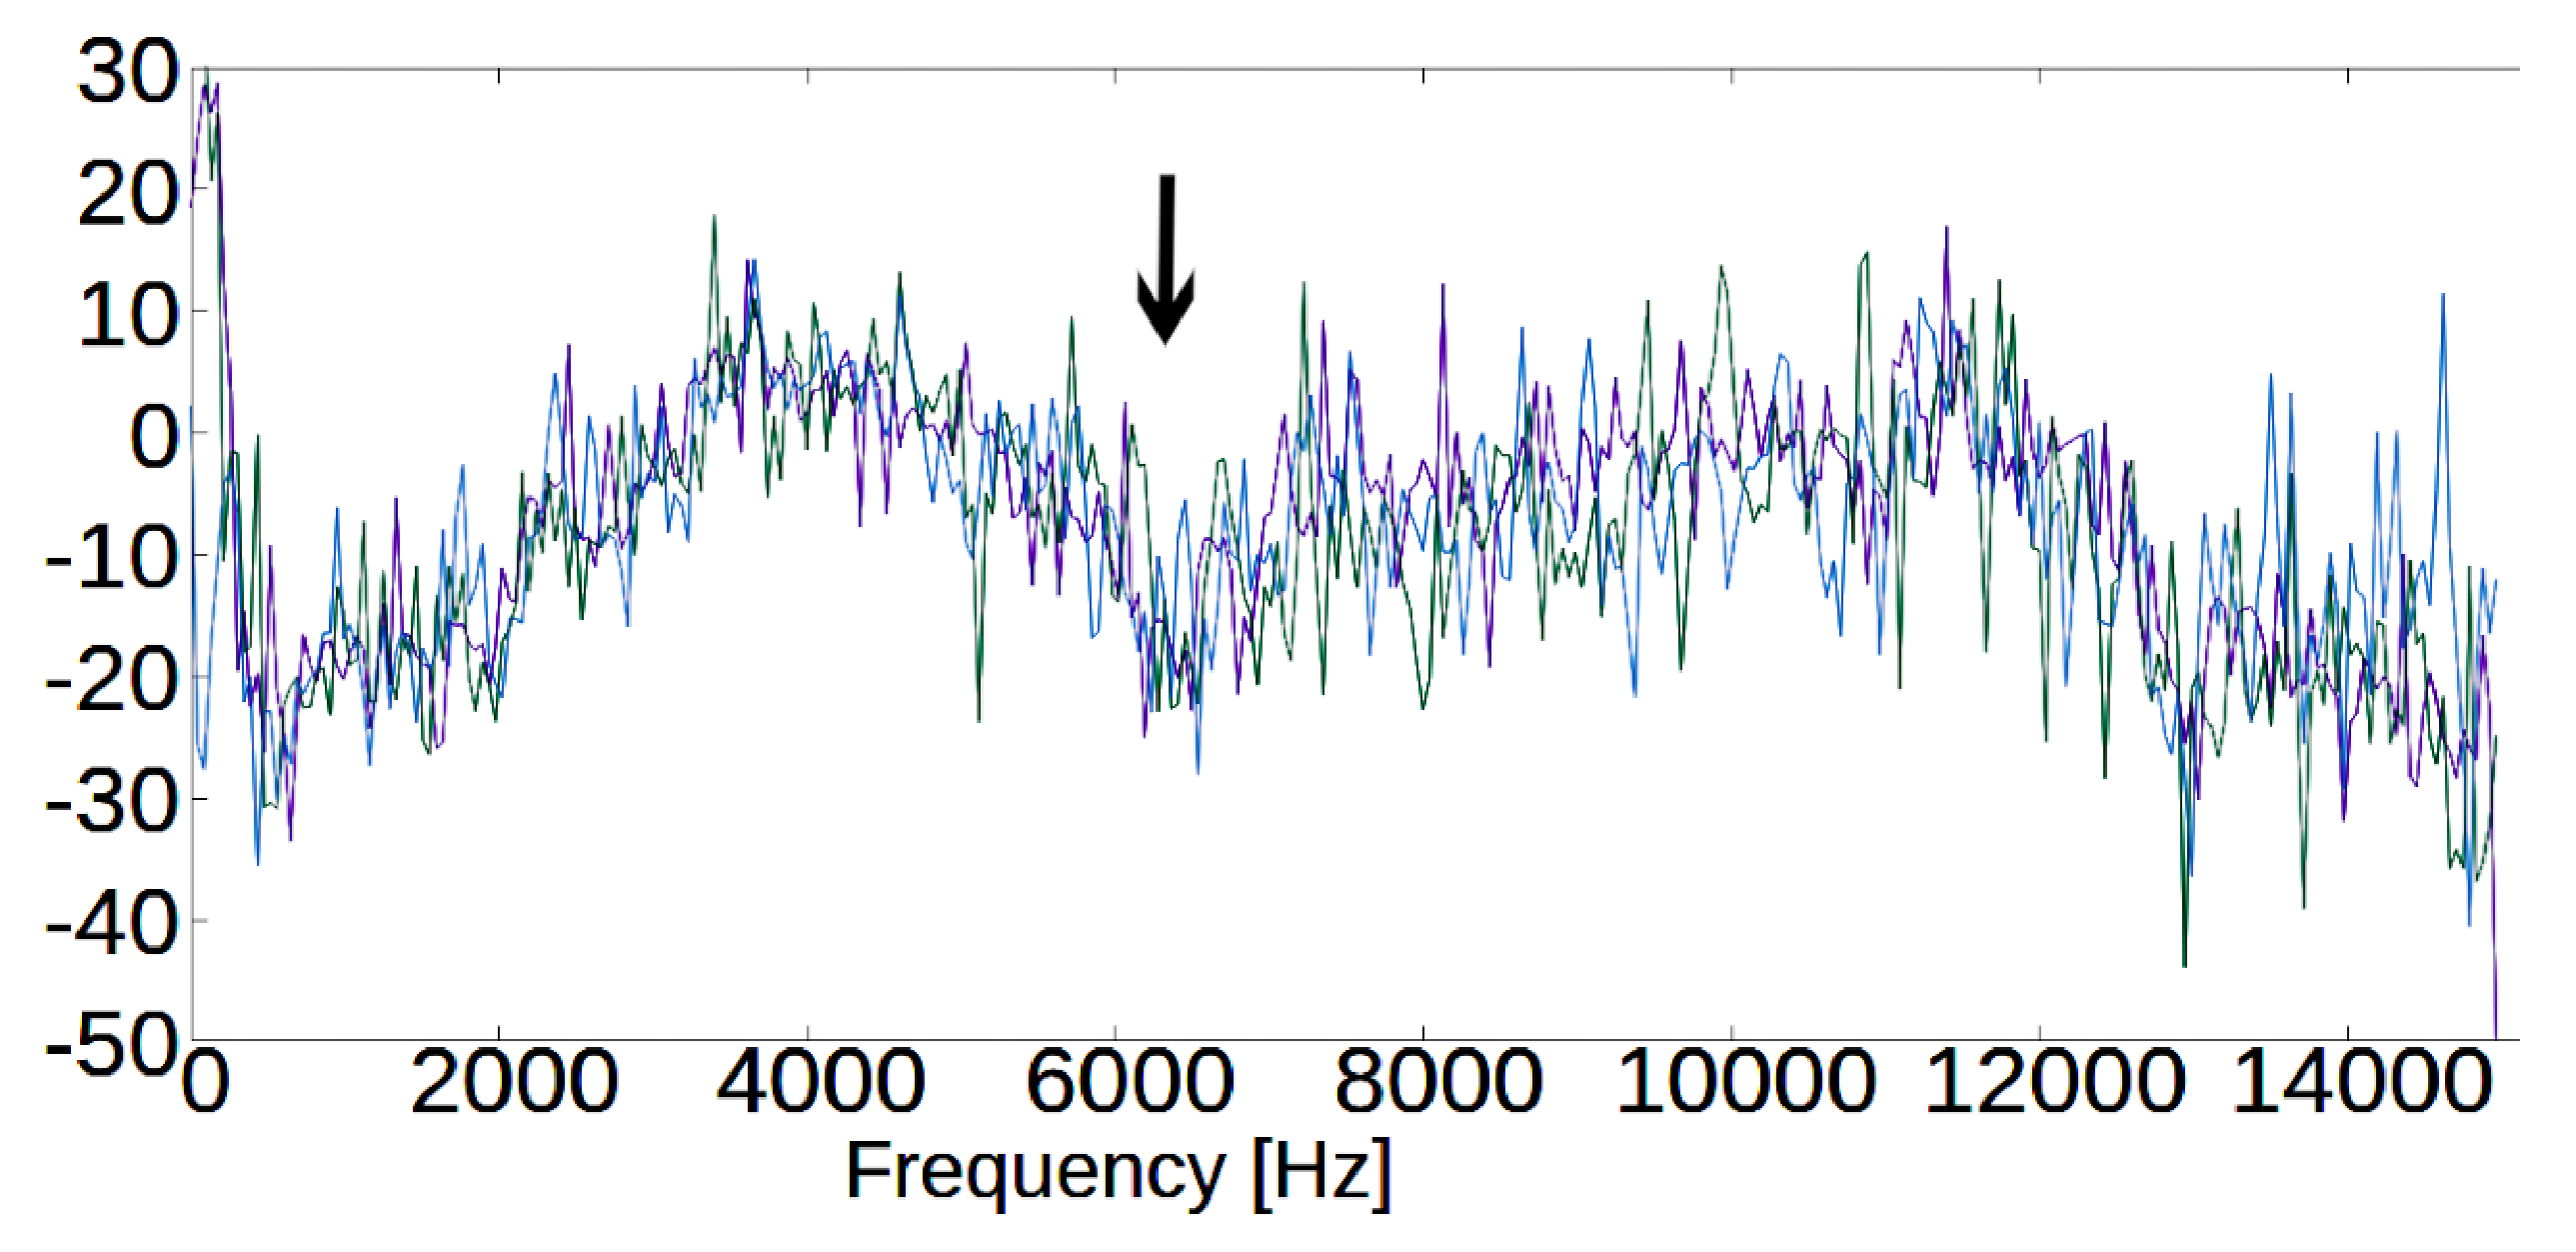
\includegraphics[keepaspectratio, scale=0.14]{picture/No1-3_mae_r.eps}
      \subcaption{音源が前方で右耳の場合}
     
    \end{minipage} \\
 
    \begin{minipage}[t]{0.45\hsize}
      \centering
      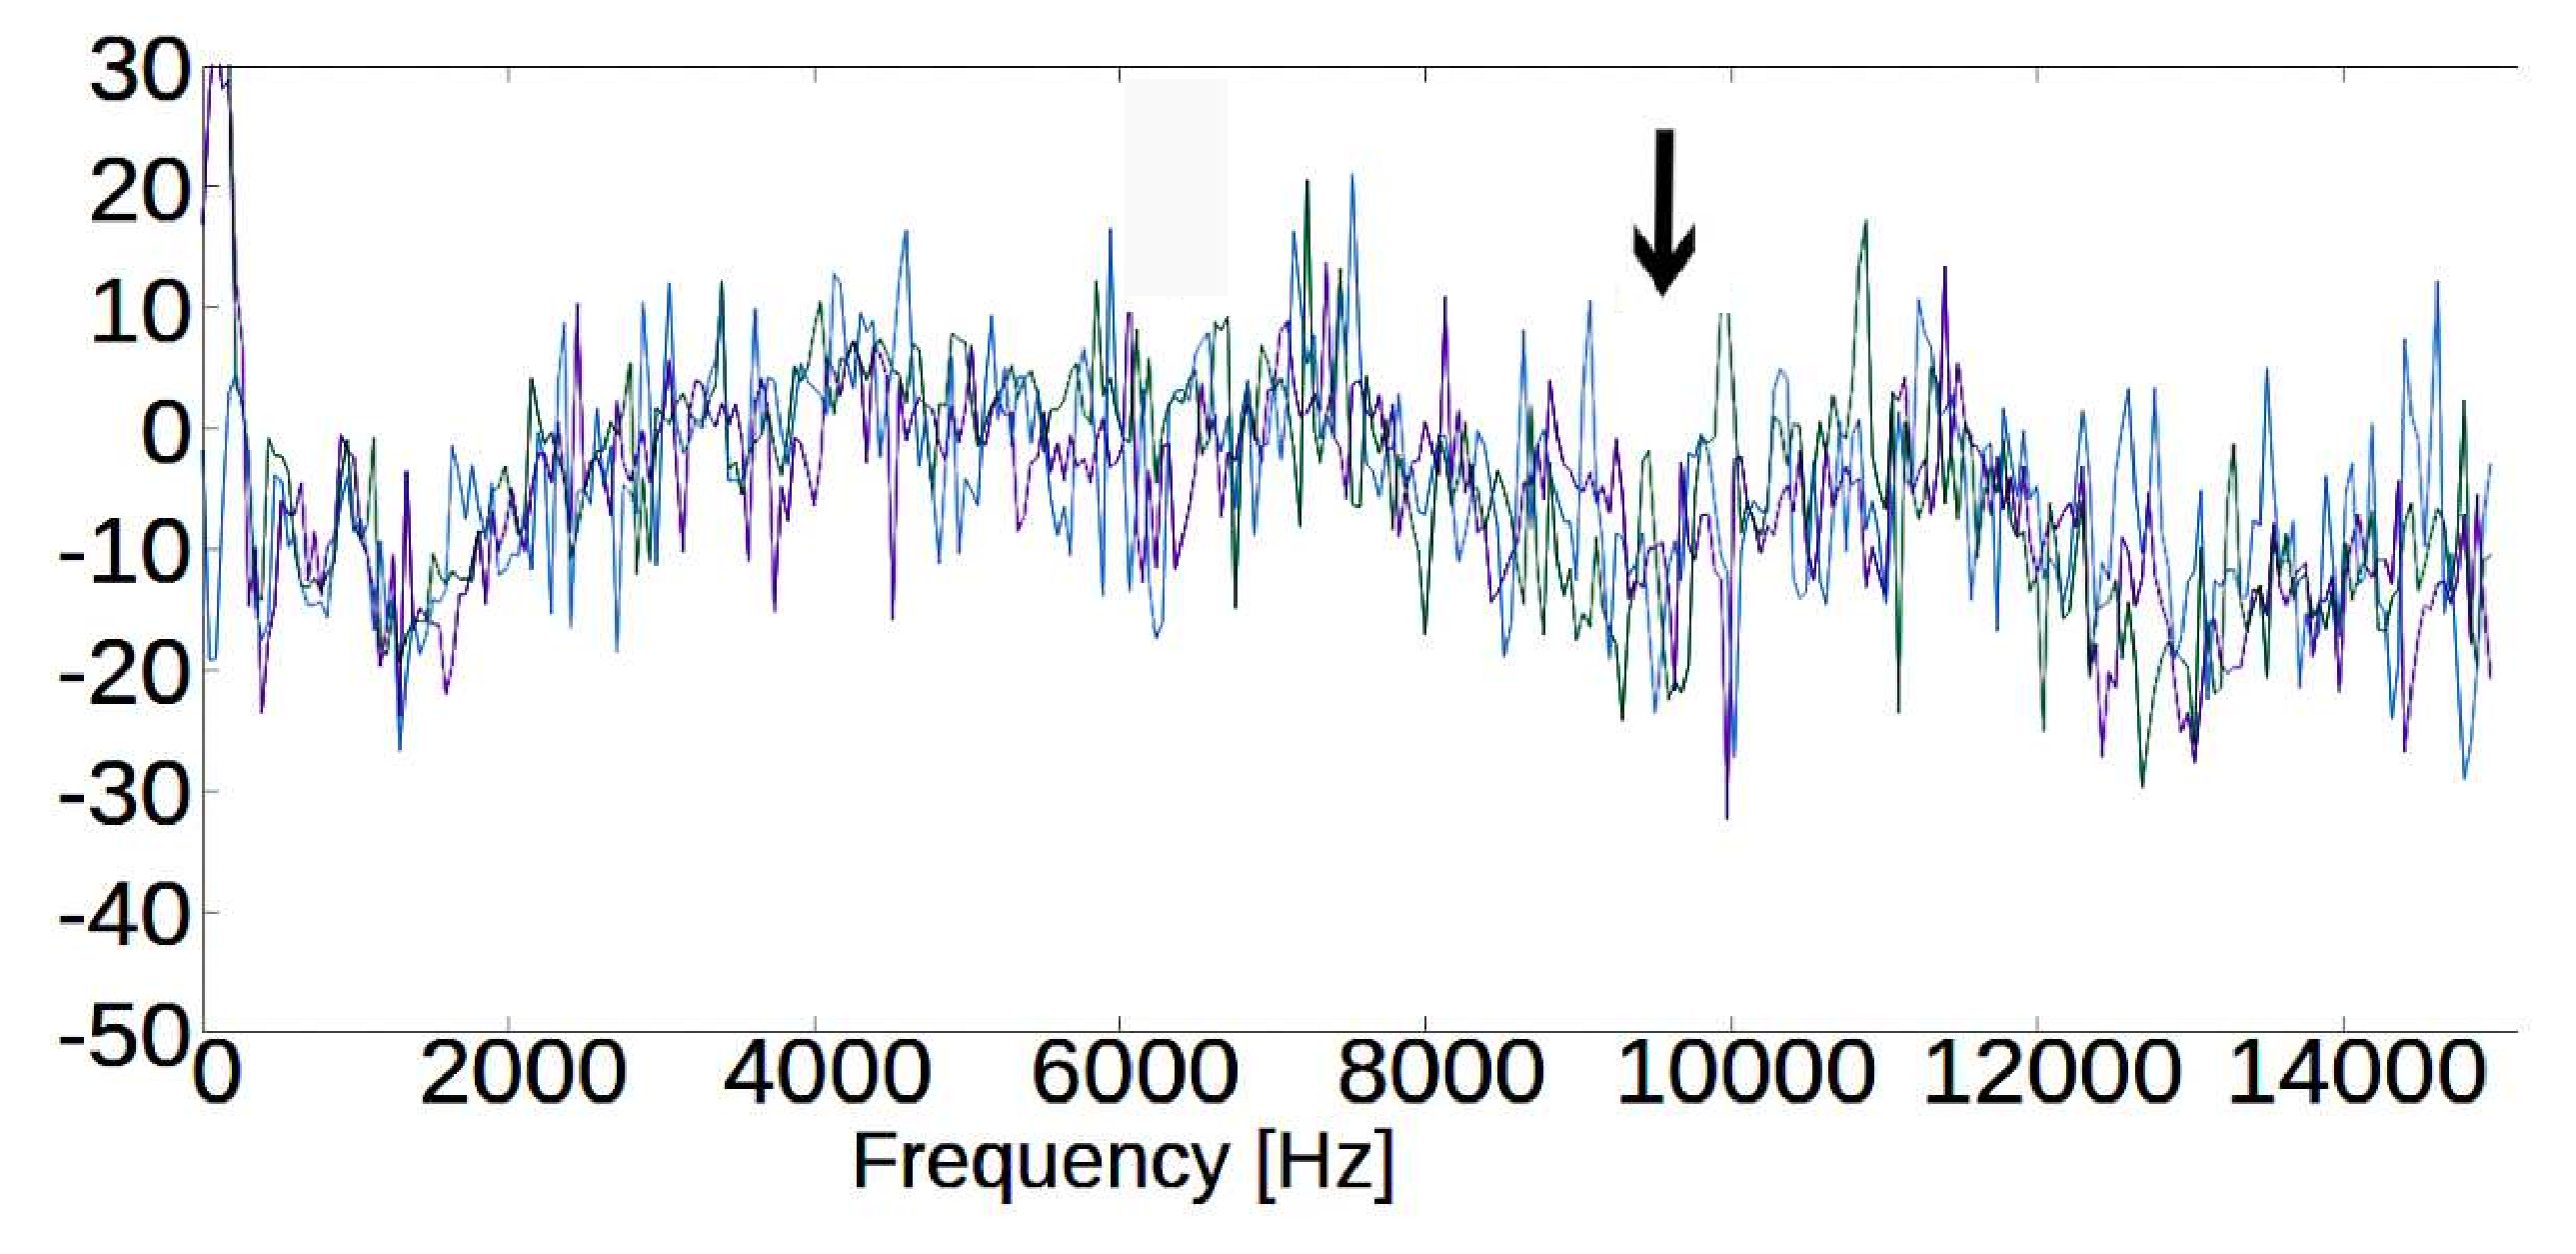
\includegraphics[keepaspectratio, scale=0.14]{picture/No1-3_usiro_l.eps}
      \subcaption{音源が後方で左耳の場合}
   
    \end{minipage} &
    \begin{minipage}[t]{0.45\hsize}
      \centering
      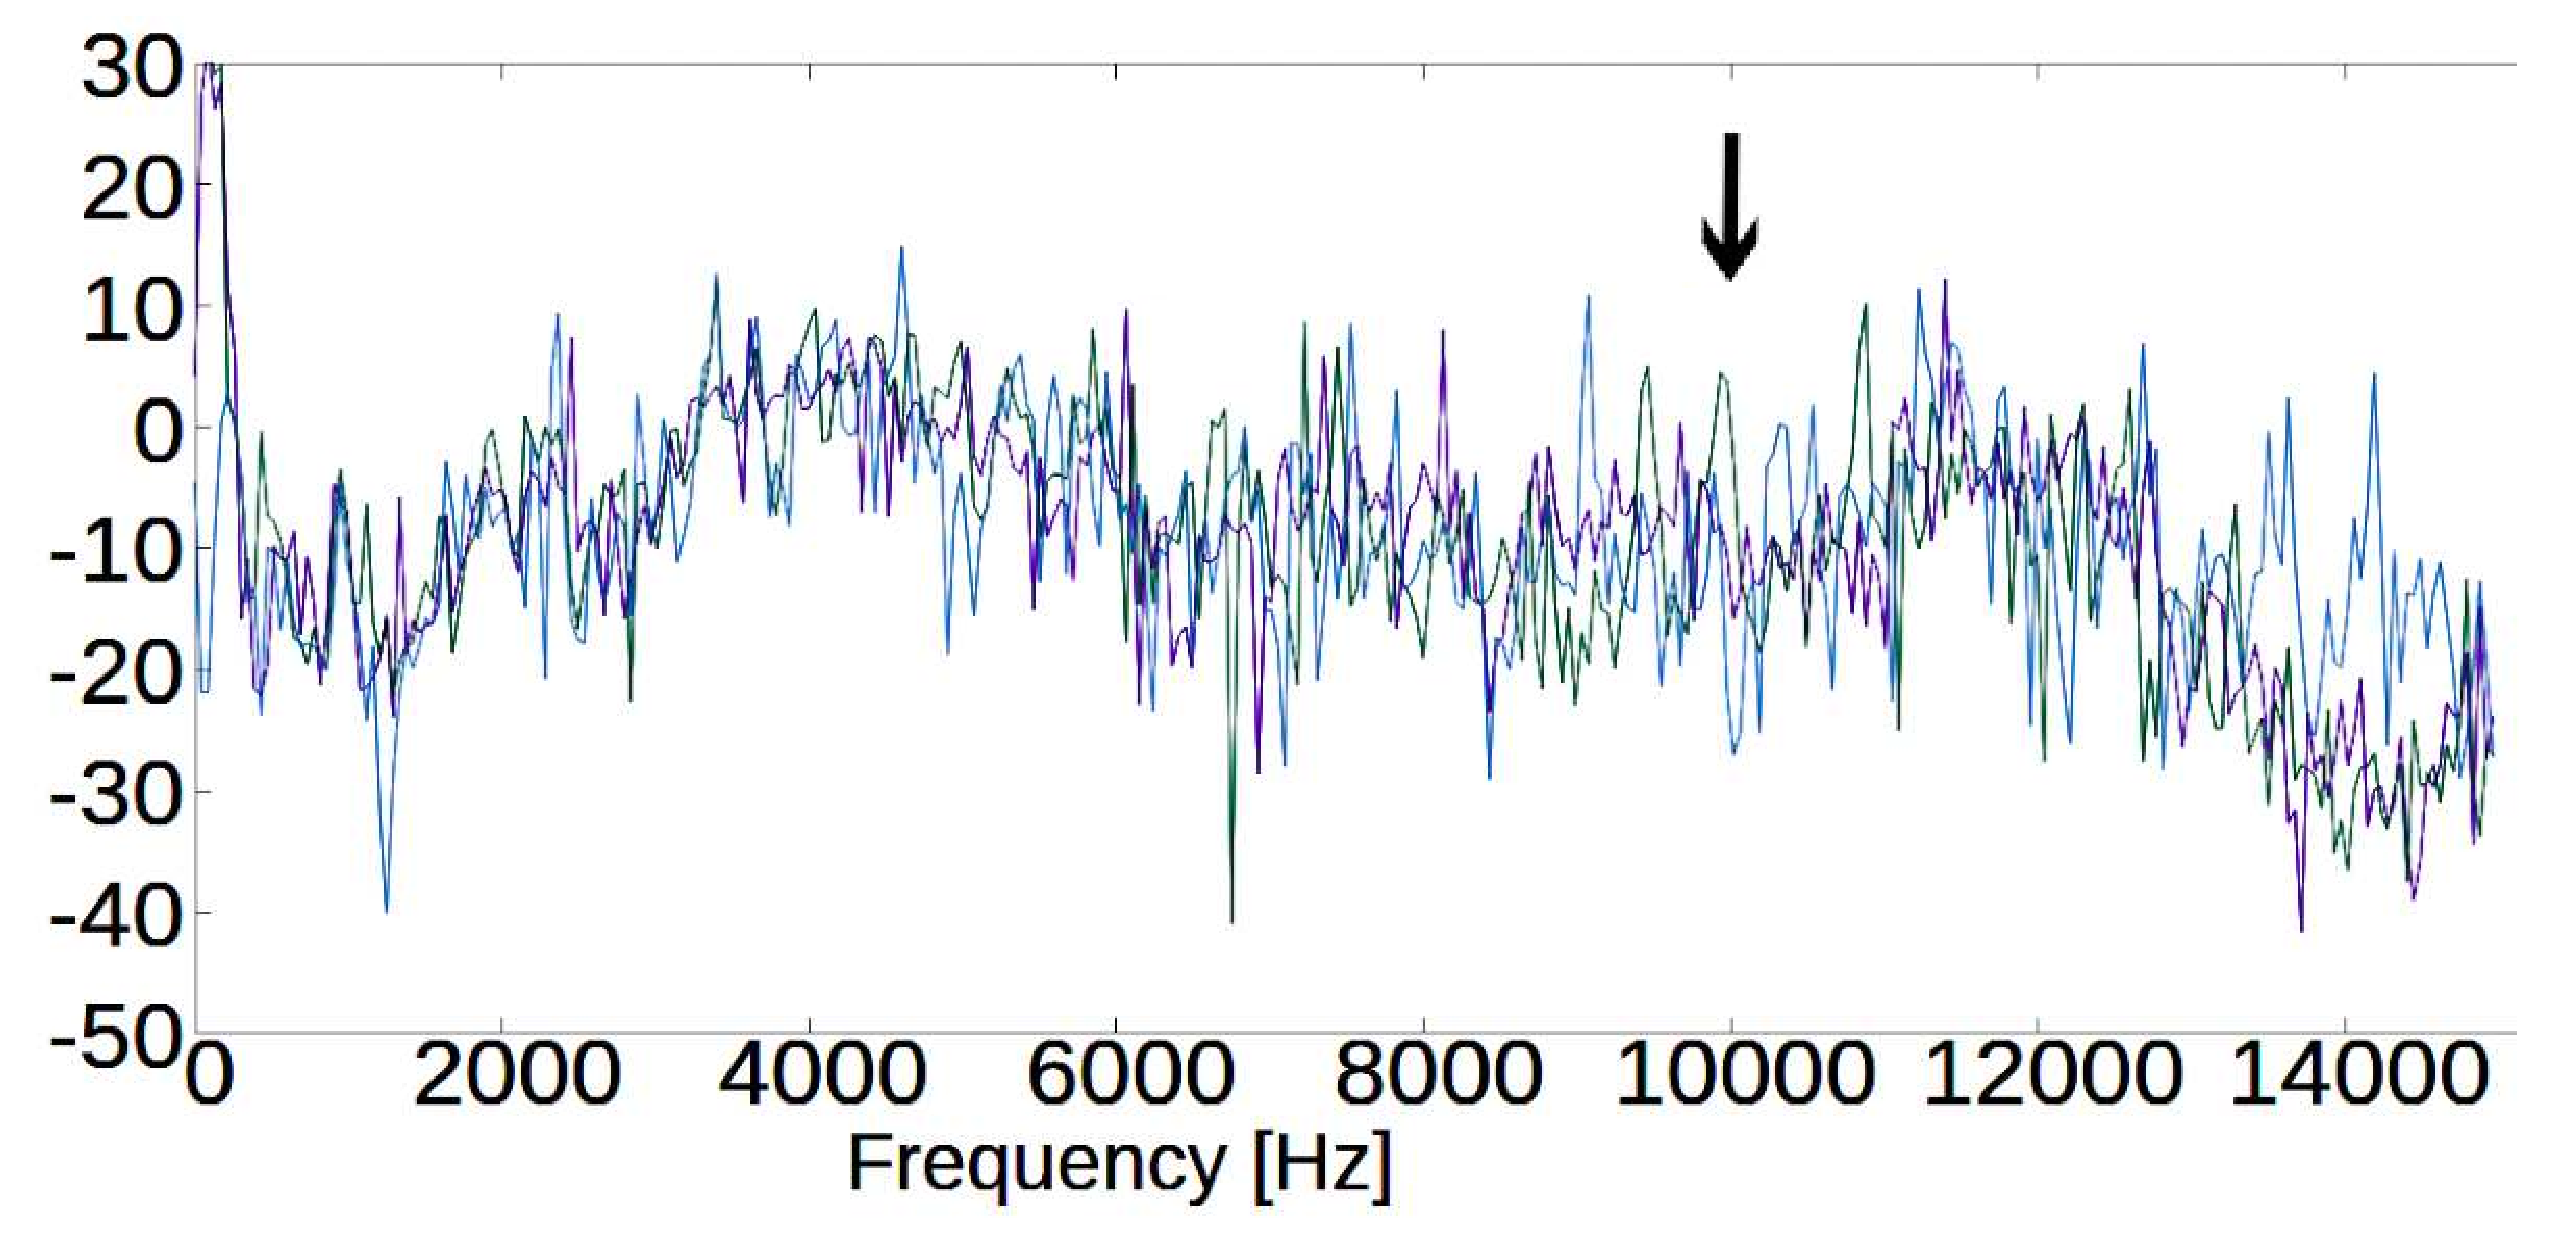
\includegraphics[keepaspectratio, scale=0.14]{picture/No1-3_usiro_r.eps}
      \subcaption{音源が後方で右耳の場合}
        \end{minipage} 
  \end{tabular}
   \caption{雑用重畳録音信号から測定した頭部伝達関数}\label{fig:HRTF}
\end{figure}

\clearpage

\section{前後の両耳間レベル差の測定}
ILDもHRTFと同様に、左耳の録音信号と右耳の録音信号から1024点のDFTによる
クロススペクトル法を用いて算出した。
計算式を式\ref{formula:ILD}に示す。
添字の$_l,_r$は各々左右の耳を表し、
$X$は背景雑音を加えた録音信号を1024サンプルでDFTした512サンプルの複素数である。

  \begin{equation}
      %ILDl,r(w) = El(w)/ Er(w)
      ILD(k) = \frac{\overline{ X_l(k)*X_r(k)^{*} }}{ \overline{ X_r(k)*X_r(k)^{*} }}\label{formula:ILD}
  \end{equation}
  
白色雑音の両耳間レベル差を図\ref{fig:whitenoiseILD}に、
220の信号ごとに得られた両耳間レベル差のうち例として3つを図\ref{fig:AILD}に示す。
図\ref{fig:whitenoiseILD}と図\ref{fig:AILD}を比べると、
どちらも10kHz付近で前後の差異が確認できた。

%\clearpage

%ILD
\begin{figure}[htbp]
  \begin{center}
       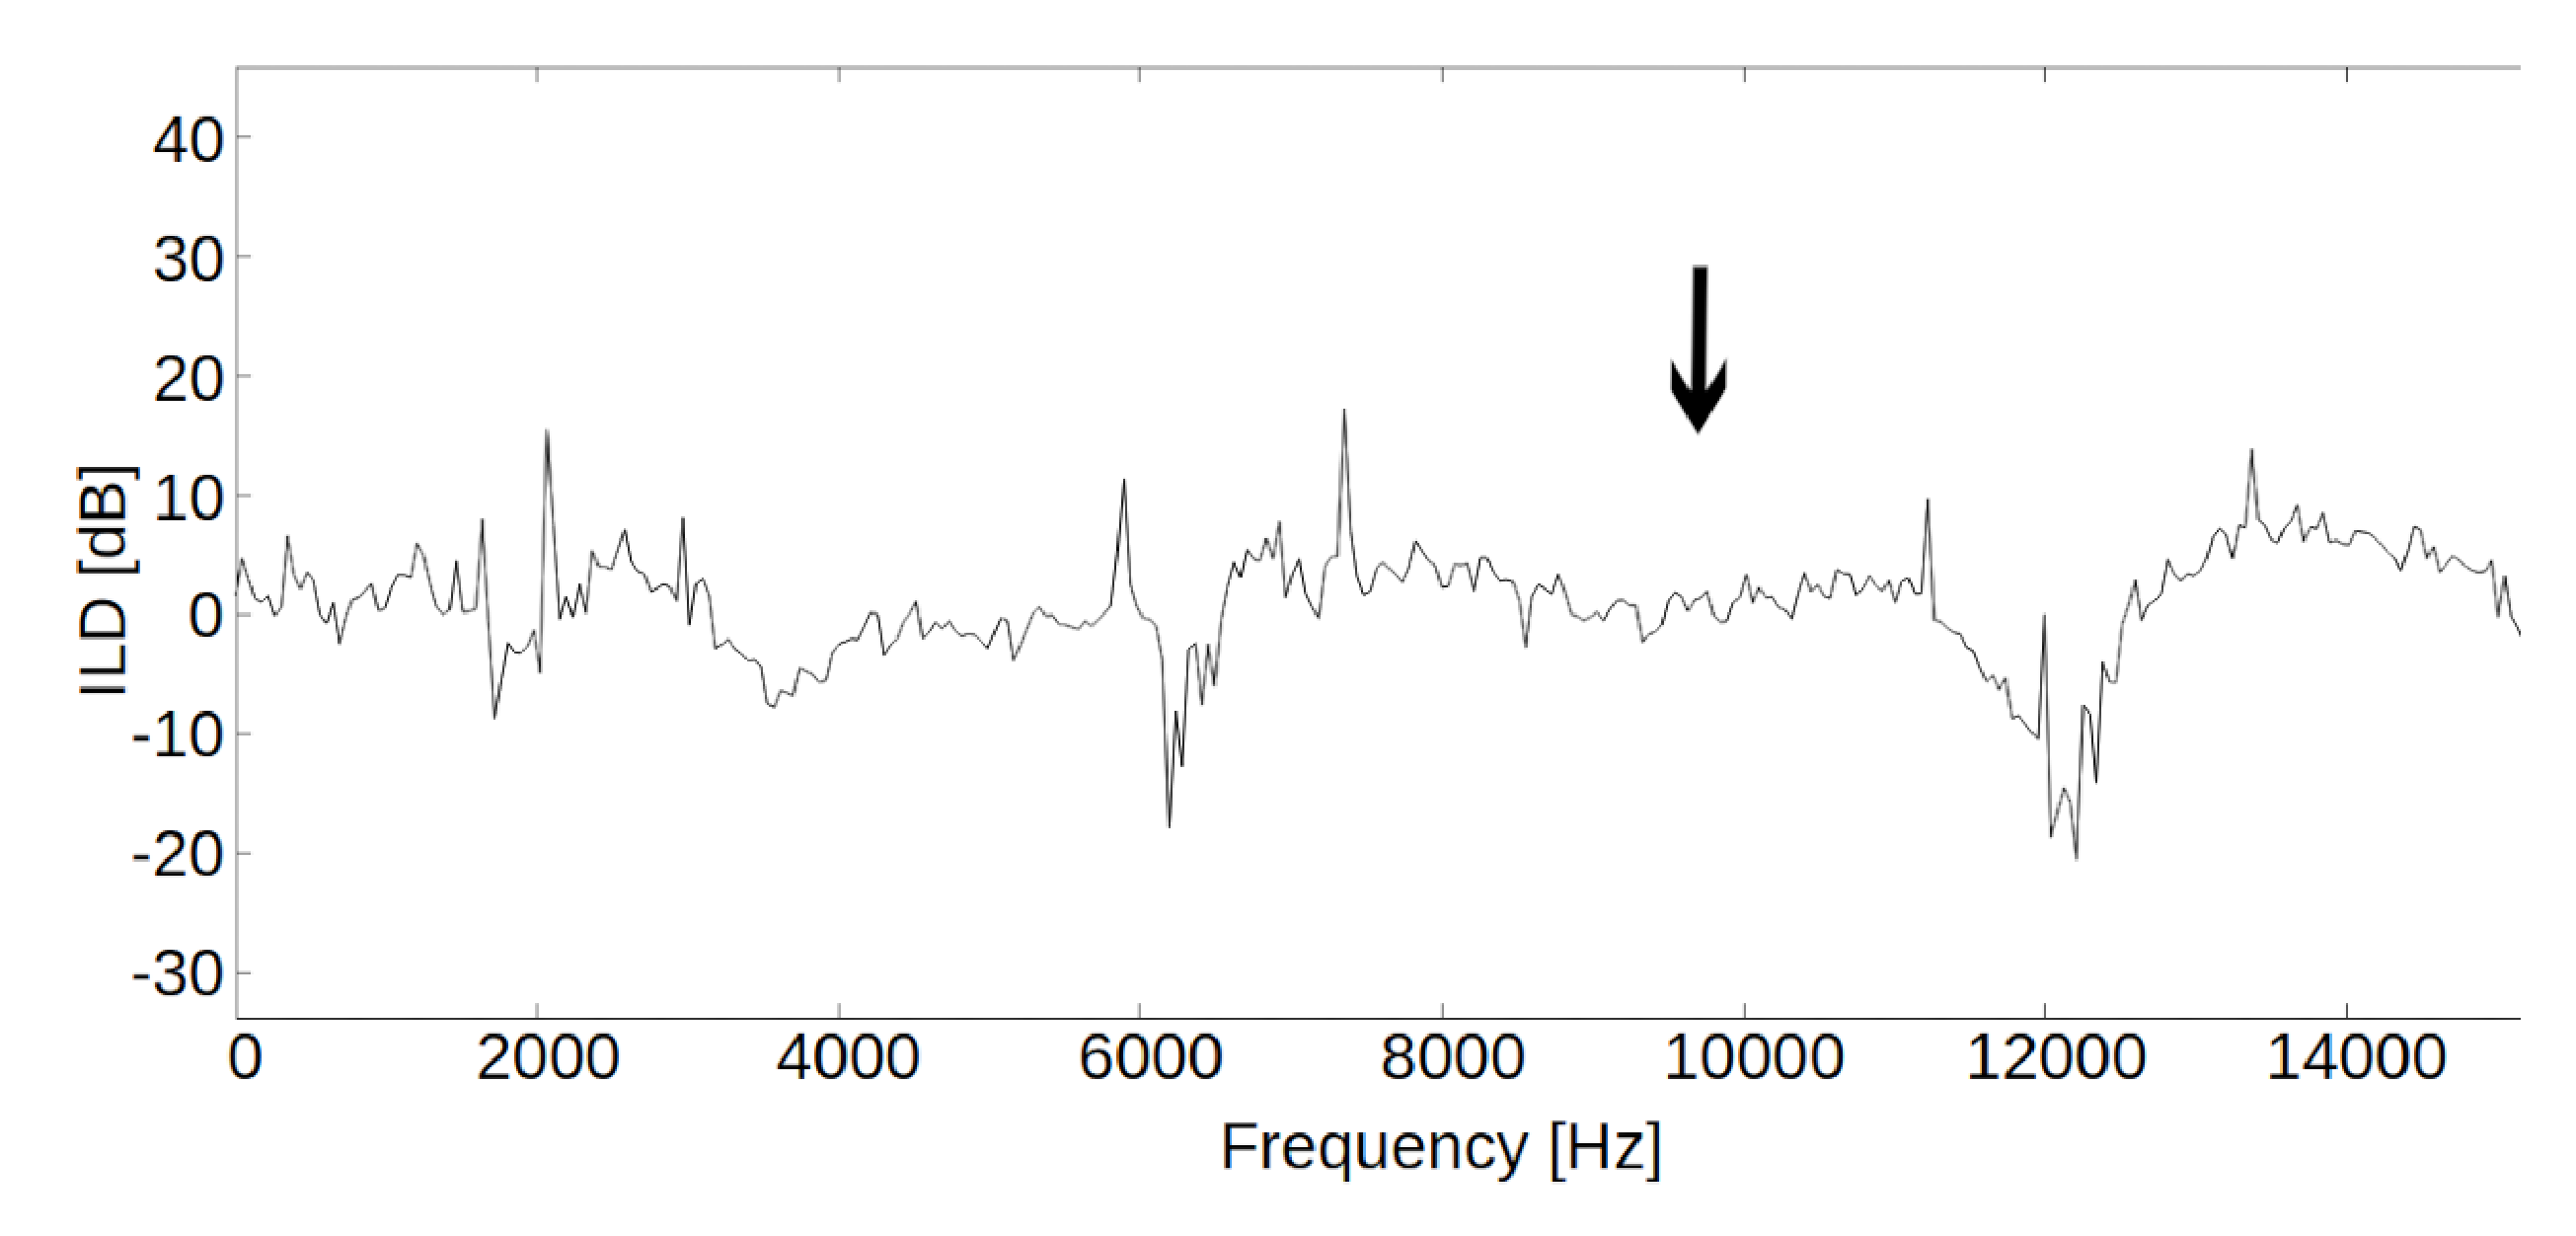
\includegraphics[clip, width=2.5in, height = 1.3in]{picture/mae_full_whitenoise.eps}
       \subcaption{音源が前方の場合}
       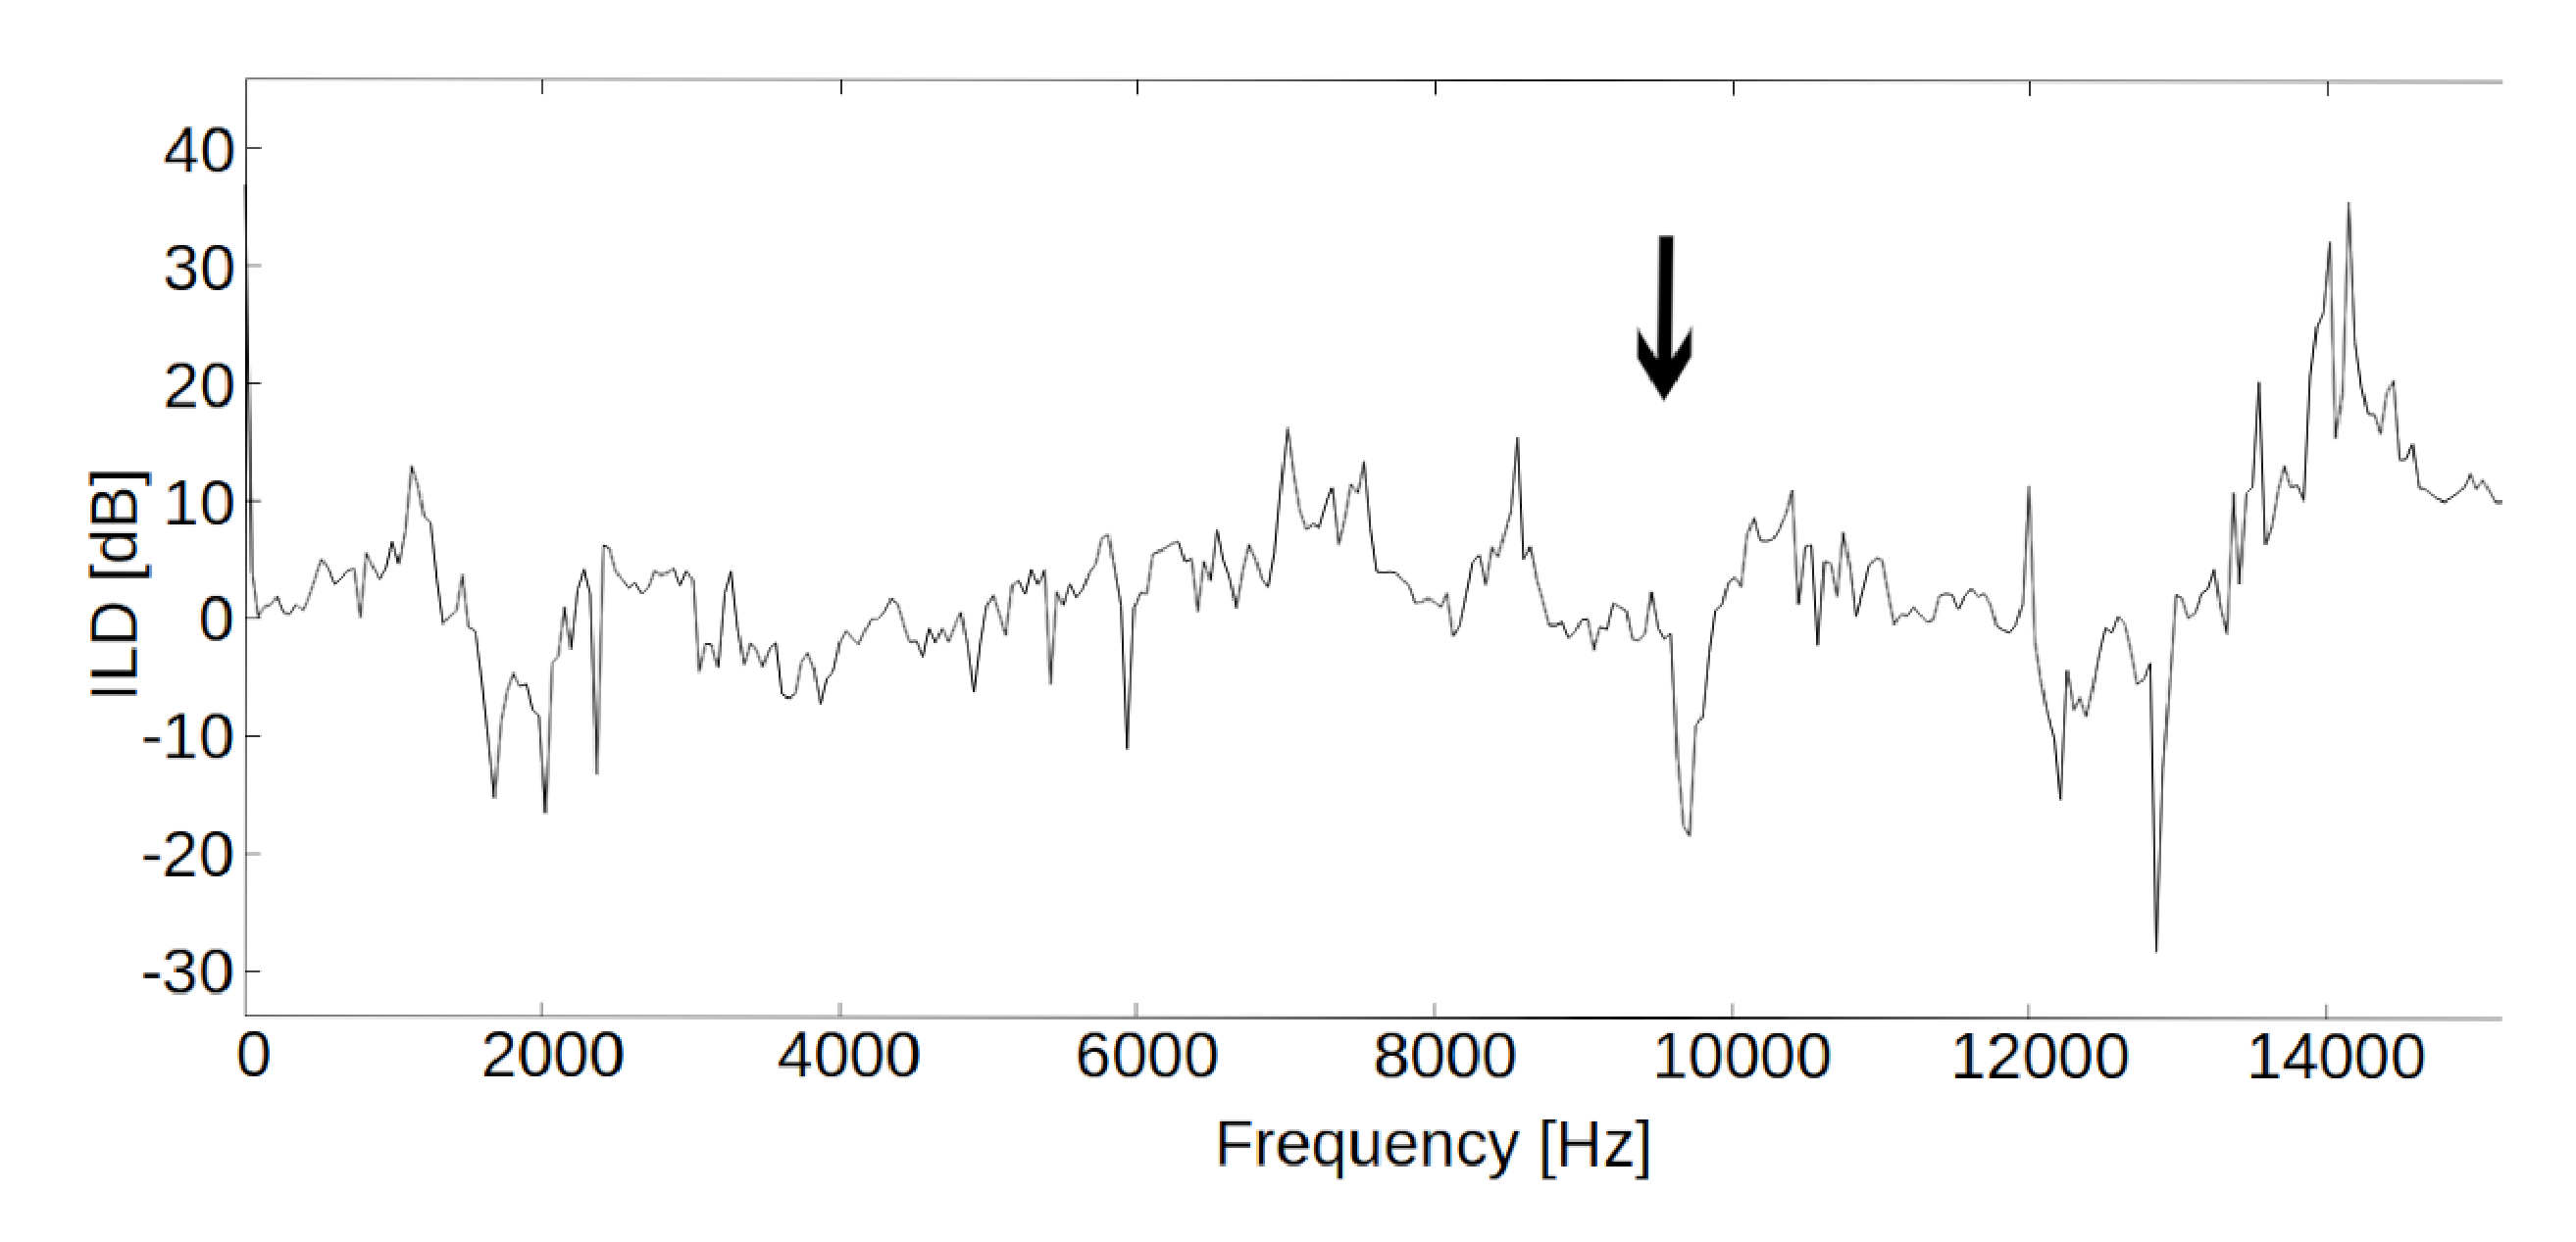
\includegraphics[clip, width=2.5in, height = 1.3in]{picture/usiro_full_whitenoise.eps}
       \subcaption{音源が後方の場合}
       \end{center}
       \caption{白色雑音を用いて測定した両耳間レベル差}\label{fig:whitenoiseILD}     
%\end{figure}
%\begin{figure}[htbp]
 
  \begin{center}
  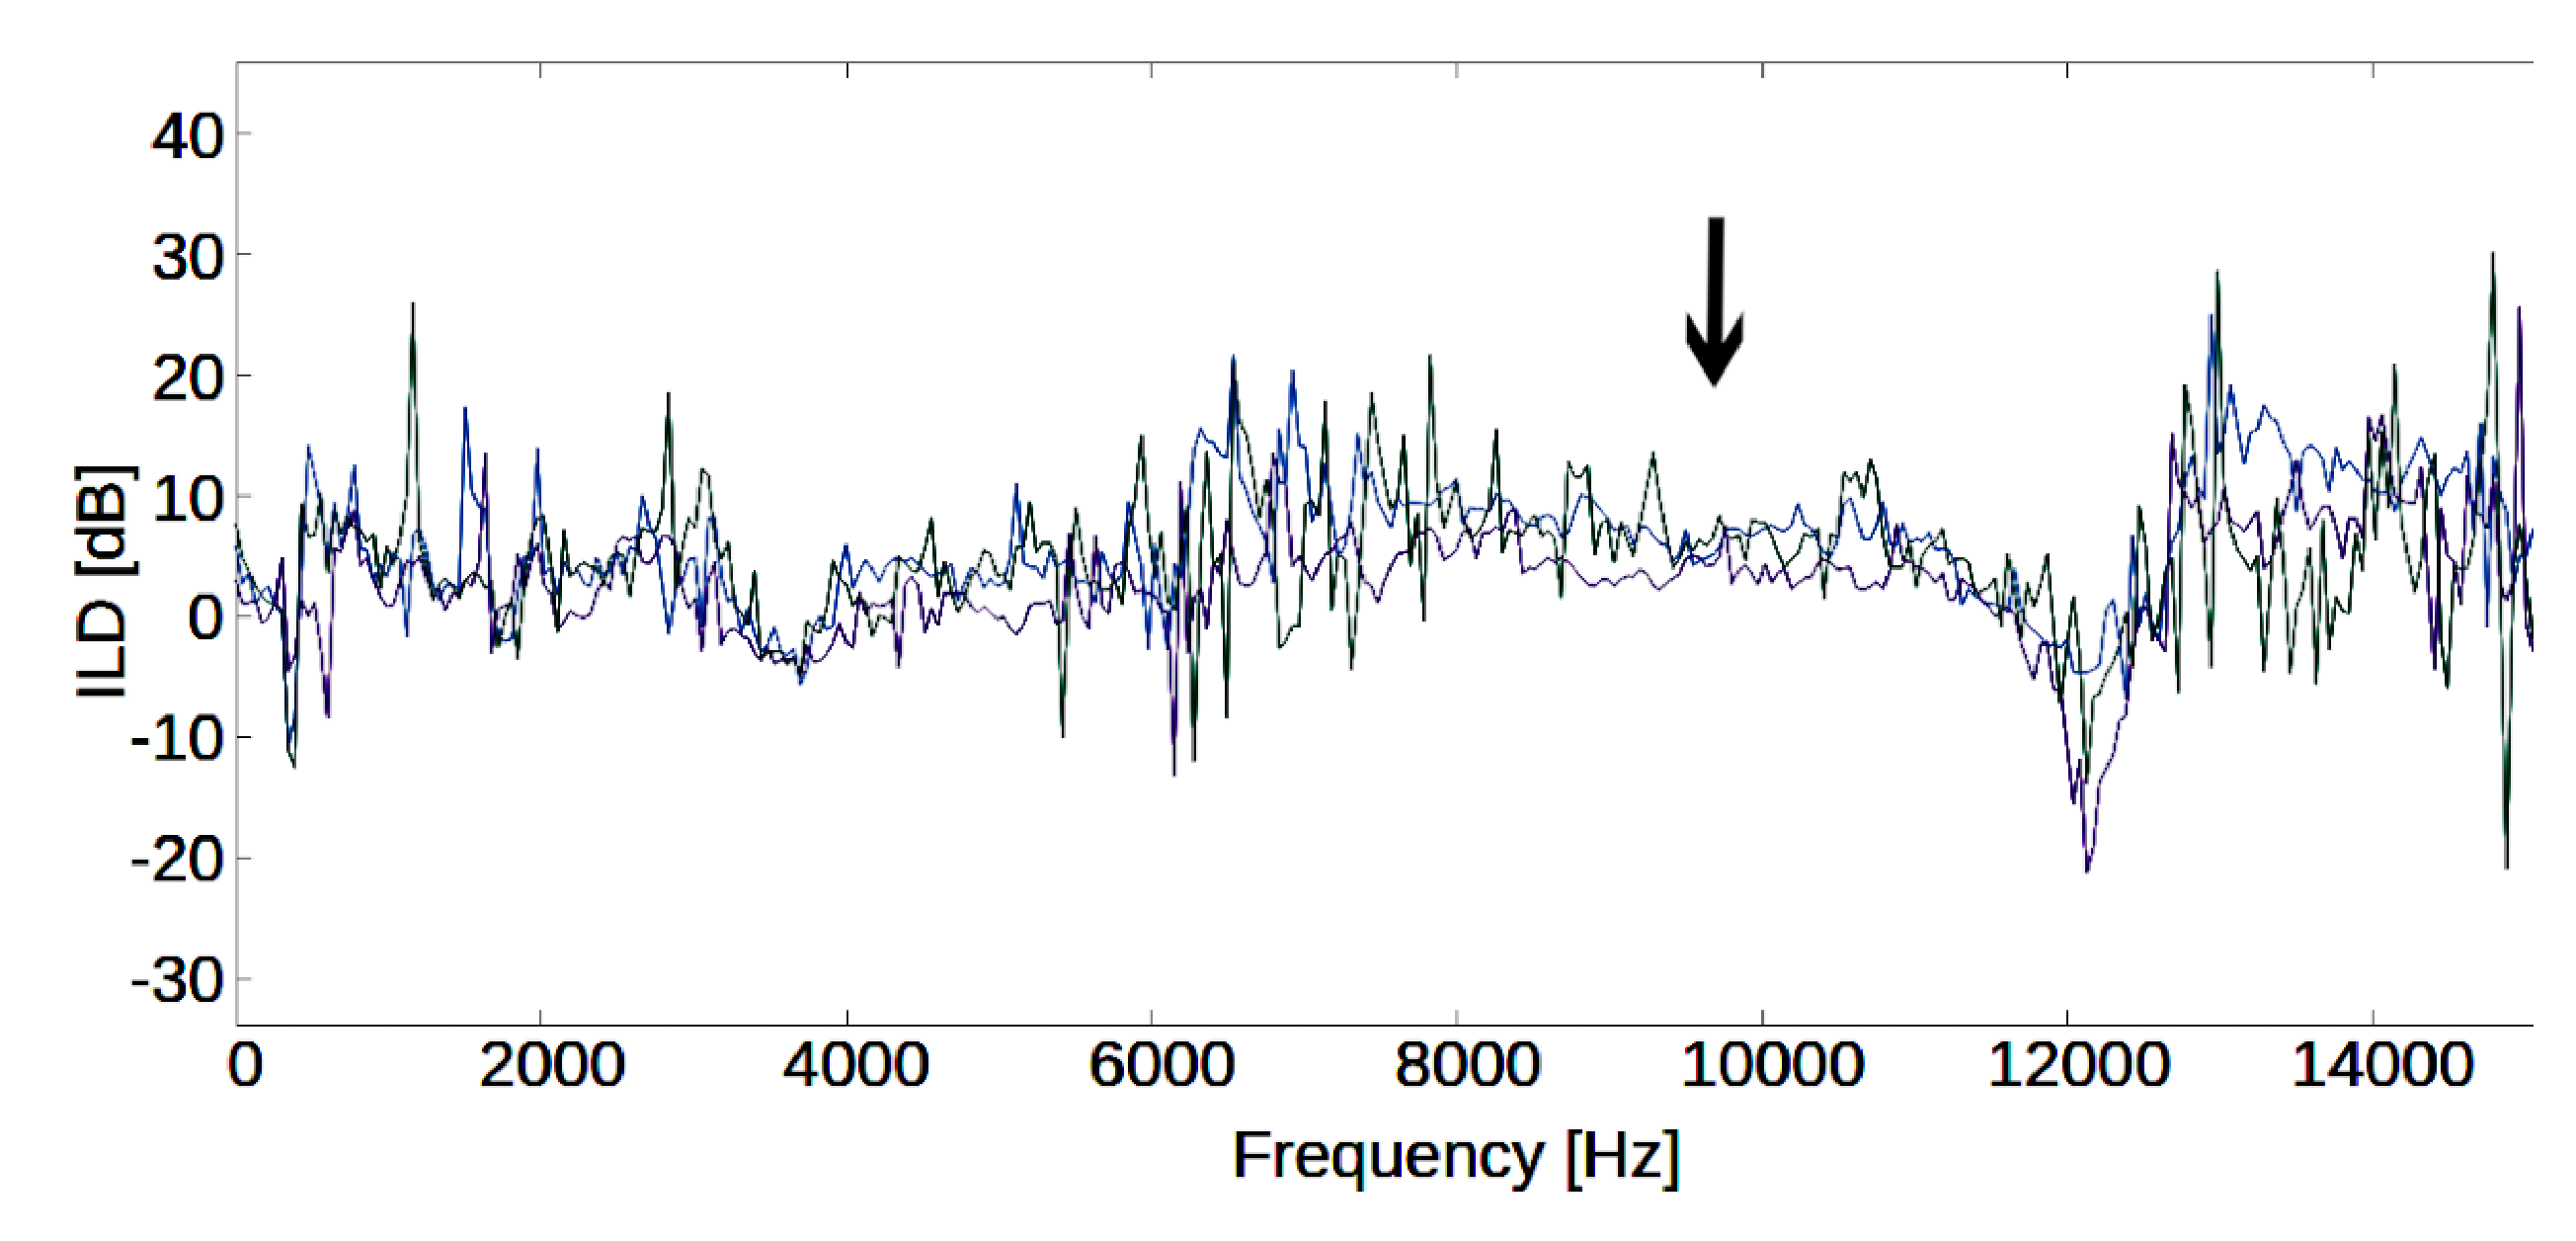
\includegraphics[clip, width=2.5in, height = 1.3in]{picture/mae_full_NoSmoothing.eps}
  \subcaption{音源が前方の場合}
  
  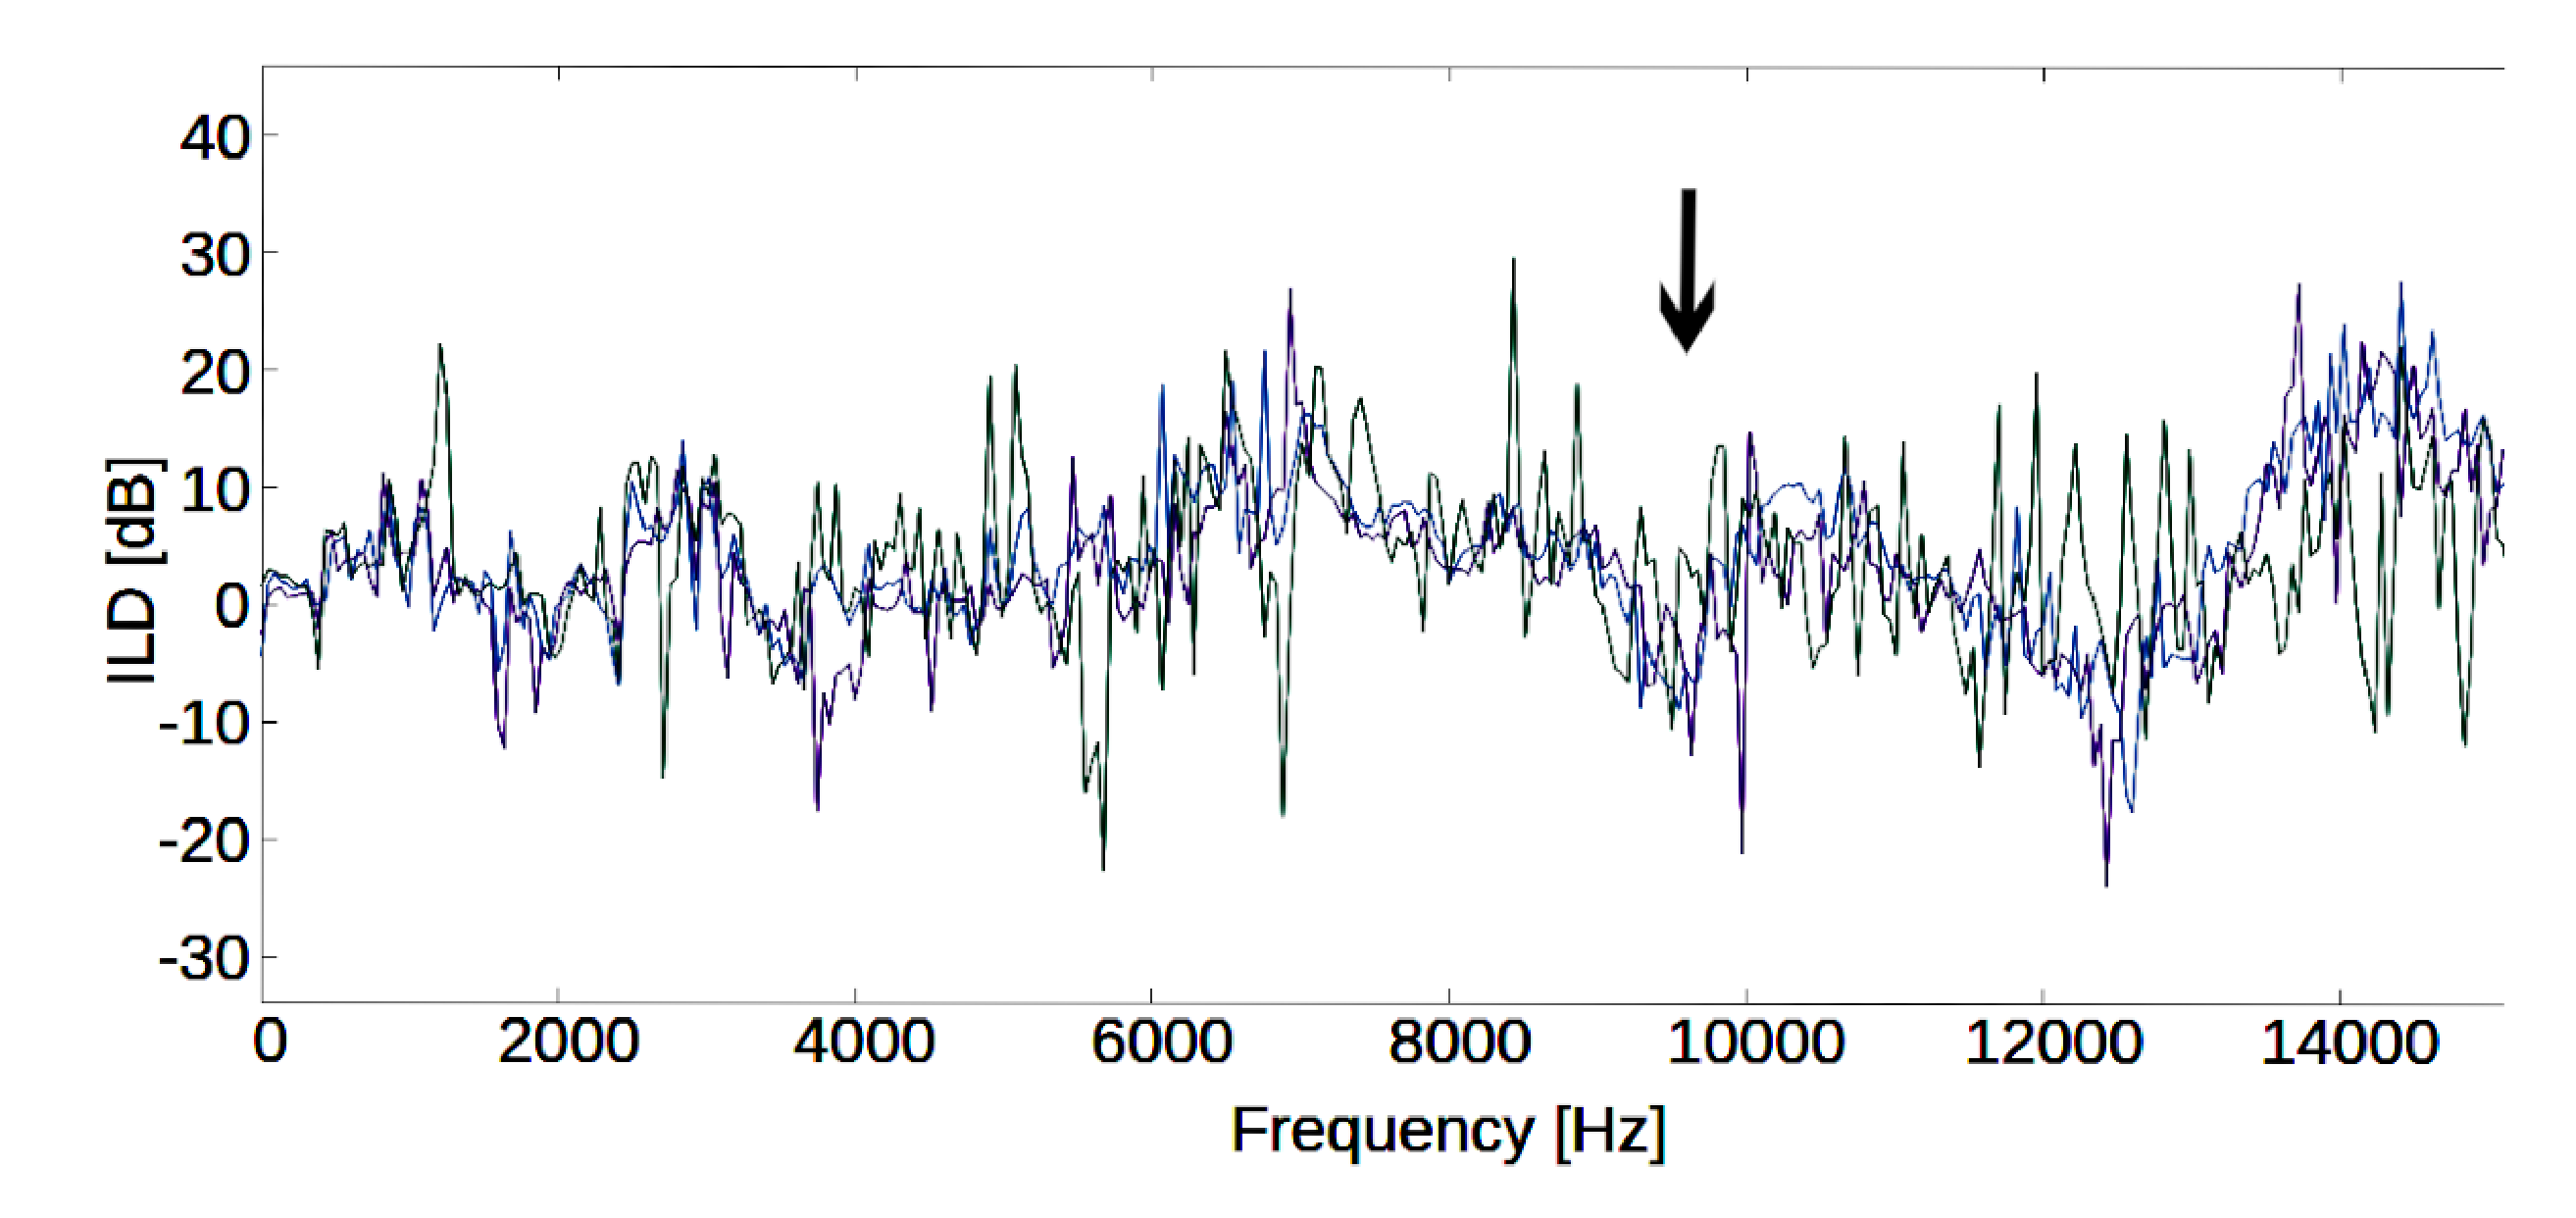
\includegraphics[clip, width=2.5in, height = 1.3in]{picture/usiro_full_NoSmoothing.eps}
  \subcaption{音源が後方の場合}
  \end{center}
  \caption{雑用重畳録音信号から測定した両耳間レベル差の例}\label{fig:AILD}
\end{figure}


%%%% リップノイズの検出
\chapter{識別テスト}\label{chap3}

\section{識別テストの方法}\label{chap3:method}
HRTFによる識別では、前後の差異が目視でも確認できた4〜12kHzの帯域を使用し、
ILDの場合では8〜15kHzの帯域を使用した。次元数は各々186点、163点であり、
教師データ220、評価データ110、
テストデータ110で機械学習を行った。
機械学習には、中間層1層のニューラルネットワークを使用し、
ラベルは音源が前方にある場合のHRTFとILDに0を、
後方にある場合のHRTFとILDには1を付与している。
また、使用したニューラルネットワークの設定は下記に示す。

\begin{itemize}
   \item 重みの初期値: 標準偏差0.01のガウス分布
   \item 活性化関数:ReLU
   \item 出力:ソフトマックス関数
\end{itemize}


\section{識別テストの結果と考察}\label{chap3:snd}
まず、評価データを用いてパラメータ(学習回数と中間層のノード数)を変化させた識別率の推移を求め、
その結果を図\ref{fig:ParameterChange_HRTF}、図\ref{fig:ParameterChange_ILD}に示す。
HRTFの場合は、パラメータを10から150まで10回刻みで変化させた識別率(10回試行の平均)の推移である。
左右の耳各々でパラメータが50のときに識別率が最も高かった。
一方、ILDの場合はパラメータを1から20を1回刻みで識別率(10回試行の平均)の推移を求めた。
その結果、パラメータが15の時に識別率が最も高かった。

次に、先の結果で識別率が最も高かったパラメータで左右のHRTF及び、ILDの識別率を10回ずつ求め、
その結果を表\ref{tab:3.1}、表\ref{tab:3.2}、表\ref{tab:3.3}に示す。
%識別実験の結果を表\ref{tb:fugafuga2}に示す。
%その結果、HRTFでは左右共に識別率50%付近、ILDでは識別率92%〜95.5%という結果になった。
この結果からHRTFを用いた場合は前後の識別が困難であり、
これは左右のHRTFどちらも同じ結果となった。
対して、ILDによる識別の場合は識別率が94.1\%となり、
教師データが220個と比較的少ない現段階では十分識別できたといえる。

最後に到来音そのものでの識別率を求めた、その結果を表\ref{tab:3.4}、表\ref{tab:3.5}に示す。
ここで到来音そのものとは、背景雑音を加えた録音信号に対し1024点のDFTスペクトルにより得られた512点の複素数
である。
結果として、左右どちらでも前後の識別が困難であることが分かった。
到来音そのものでもこの結果ということは、到来音よりも優位なHRTFでも先の結果となることは妥当な結果であると言える。

\begin{figure}[htbp]
  \begin{tabular}{cc}
    \begin{minipage}[t]{0.5\hsize}
      \centering
      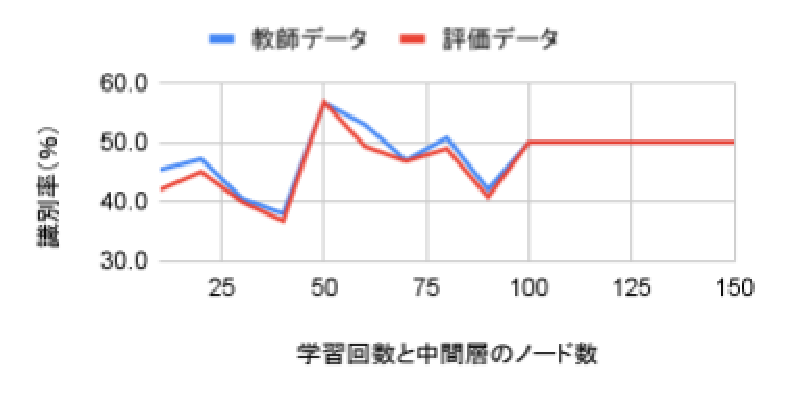
\includegraphics[clip, width=2.7in, height = 1.5in]{picture/ParameterChange_HRTF_Left.eps}
      \subcaption{左耳の場合}

    \end{minipage} &
    \begin{minipage}[t]{0.5\hsize}
      \centering
      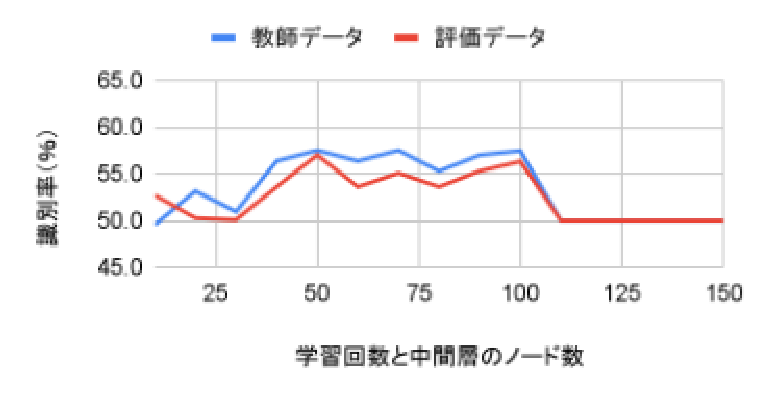
\includegraphics[clip, width=2.7in, height = 1.5in]{picture/ParameterChange_HRTF_Right.eps}
      \subcaption{右耳の場合}
     
    \end{minipage} \\
 
  \end{tabular}
   \caption{パラメータの変化によるHRTFの識別率の推移}\label{fig:ParameterChange_HRTF}
\end{figure}

\begin{figure}[htbp]
  \begin{center}
  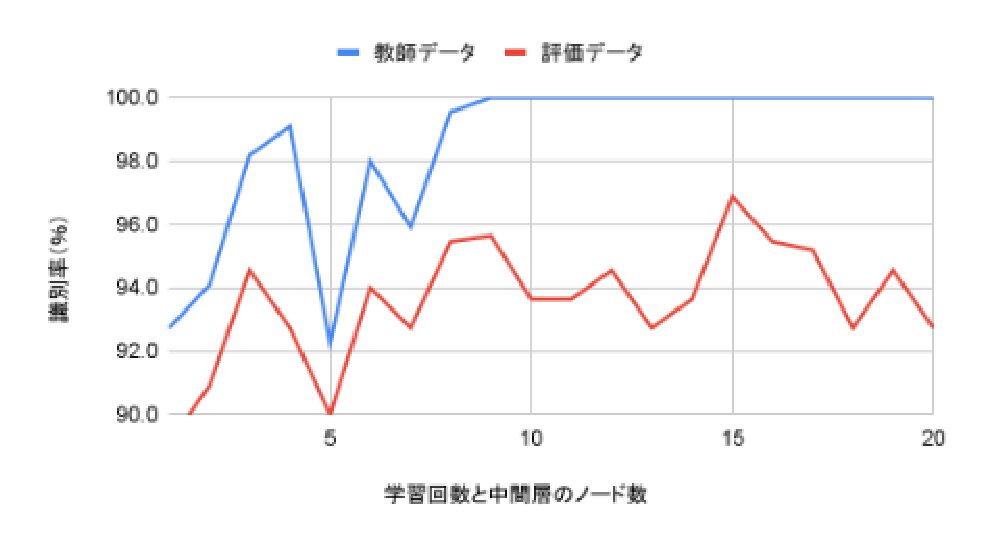
\includegraphics[clip, width=3.0in, height = 1.5in]{picture/ParameterChange_ILD.eps}
  \end{center}
  \caption{パラメータの変化によるILDの識別率の推移}\label{fig:ParameterChange_ILD}
  \end{figure}

  \clearpage

  \begin{table}[!htp]\centering
    \caption{HRTF(左)の学習回数50、中間層のノード数50での識別率}\label{tab:3.1}
    \scriptsize
    \begin{tabular}{l|rrrrrrrrrrr}
    &1 &2 &3 &4 &5 &6 &7 &8 &9 &10 \\
    \hline
    教師データの認識率(%) &62.3 &53.6 &70.0 &70.0 &50.0 &36.8 &36.8 &50.0 &49.5 &39.5 \\
    テストデータの認識率(%) &60.0 &57.4 &69.2 &69.2 &51.9 &39.3 &39.3 &51.9 &52.8 &43.7 \\
    \hline
    教師データの認識率の平均(%) &51.9 & & & & & & & & & \\
    テストデータの認識率の平均(%) &53.5 & & & & & & & & & \\
    \hline
    %\bottomrule
    \end{tabular}
    \end{table}

    \begin{table}[!htp]\centering
      \caption{HRTF(右)の学習回数50、中間層のノード数50での識別率}\label{tab:3.2}
      \scriptsize
      \begin{tabular}{l|rrrrrrrrrrr}
      &1 &2 &3 &4 &5 &6 &7 &8 &9 &10 \\
      \hline
      教師データの認識率(%) &49.5 &50.0 &49.1 &49.1 &50.9 &76.8 &76.8 &50.9 &65.5 &51.8 \\
      テストデータの認識率(%) &50.0 &49.1 &48.2 &48.2 &50.9 &74.5 &74.5 &47.3 &60.9 &52.7 \\
      \hline
      教師データの認識率の平均(%) &57.0 & & & & & & & & & \\
      テストデータの認識率の平均(%) &55.6 & & & & & & & & & \\
      \hline
     \end{tabular}
      \end{table}

    \begin{table}[!htp]\centering
      \caption{ILDの学習回数15、中間層のノード数15での識別率}\label{tab:3.3}
      \scriptsize
      \begin{tabular}{l|rrrrrrrrrrr}
      &1 &2 &3 &4 &5 &6 &7 &8 &9 &10 \\
      \hline
      教師データの認識率 &100.0 &100.0 &100.0 &100.0 &100.0 &100.0 &100.0 &100.0 &100.0 &100.0 \\       
      テストデータの認識率 &93.4 &93.4 &93.4 &94.4 &94.4 &94.4 &94.4 &94.4 &94.4 &94.4 \\
      \hline
      教師データ の認識率の平均 &100.0 & & & & & & & & & \\        
      テストデータ の認識率の平均 &94.1 & & & & & & & & & \\
      \hline
      \end{tabular} 
     \end{table}

     \begin{table}[!htp]\centering
      \caption{到来音(左)そのものでの識別率}\label{tab:3.4}
      \scriptsize
     \begin{tabular}{l|rrrrrrrrrrrrr}
      学習回数と中間層のノード数 &10 &20 &30 &40 &50 &60 &70 &80 &90 &100 &110 &120 \\
      \hline
      教師データの識別率 &50.0 &50.0 &50.0 &50.0 &50.0 &50.0 &50.0 &50.0 &50.0 &50.0 &50.0 &50.0 \\
      評価データの識別率 &50.0 &50.0 &50.0 &50.3 &50.2 &50.2 &50.2 &50.0 &50.3 &49.8 &50.1 &49.9 \\
      \end{tabular}
      \end{table}

      \begin{table}[!htp]\centering
        \caption{到来音(右)そのものでの識別率}\label{tab:3.5}
        \scriptsize
        \begin{tabular}{l|rrrrrrrrrrrrr}
          学習回数と中間層のノード数 &10 &20 &30 &40 &50 &60 &70 &80 &90 &100 &110 &120 \\
        \hline
        教師データの識別率 &50.0 &50.0 &50.0 &50.0 &50.0 &50.0 &50.0 &50.0 &50.0 &50.0 &50.0 &50.0 \\
        評価データの識別率 &50.0 &50.0 &50.0 &50.0 &50.0 &50.3 &50.0 &49.9 &49.8 &49.9 &50.1 &49.7 \\
        \end{tabular}
        \end{table}
  

\clearpage

\begin{comment}
  \begin{table}[htbp]
  \centering
  \begin{tabular}{l|c|c|c}
    & HRTF(左) & HRTF(右) & ILD \\\hline
          テストデータの識別率 & 53.5 & 55.6 &  94.1 \\
          評価データの識別率 & 56.8 &57.0& 96.9  \\ 
          教師データのみの識別率 & 56.7 & 57.0 &  100  \\
          学習回数 & 50 & 50 & 15  \\
          中間層のノード数 & 50 & 50 & 15  \\ 
      \end{tabular}
      \caption{HRTFとILDの前後識別結果}
      \label{tb:fugafuga2}
    \end{table}
\end{comment}

\chapter{むすび}\label{chap4}

本研究では、雑音下での断片的な信号からのHRTFとILDの機械学習を用いた前後方向の識別を行った。
その結果、到来音そのものよりも有利な
HRTFの場合でも識別率53.5%と識別が困難であり、対して聴覚において両耳信号から計算可能なILDの場合は識別率が 94.1%と高い識別性能であった。
このことから、断片的で片寄った信号や背景雑音を含んだ信号など実世界の到来音においては
従来の研究で主張されているHRTFよりもILDによる前後の識別の方が容易である事が分かった。

学習器で識別できるということは、実世界においてヒトは両耳間の違いによって前後の差異を学習しているという
仮説が成り立つといえる。
\begin{comment}
このことから、教師データを増やす事で将来的に識別は可能であると考えられる。
つまり、学習器で識別できるという事は、ヒトも前後の差異を学習している仮説が
十分に成り立つといえる。
\end{comment}
長年、ヘッドホン受聴による音像制御が研究されているが、
特に前後の正面定位に関しては
十分な性能のシステムが実現されているとはいえない。
%本研究の結果はそれらが可能であるという裏付けになるといえる。
本研究の結果は音像制御において左右差を強調する方が前後の定位には有効かもしれないという可能性を示した。

%%%% 参考文献
\begin{thebibliography}{9}% more than 9 --> 99 / less than 10 --> 9
  % \bibitem{oldclass}
  % 卒業研究発表会サイト, 
  % 従来の卒業研究報告予稿集用クラスファイル(p{\LaTeX}専用), 
  % \url{https://blue0.an.cis.iwate-u.ac.jp/WebSite/Misc/Graduation/format.html}
  %\bibitem{M}
  %M. Morimoto and Y. Ando, J. Acoust. Soc. Jpn. (E), vol.1, pp. 167-174, 1980.
  \bibitem{K}
  K. Iida et al., Applied Acoustics, vol.68, pp.835-850, 2007.
  
  \bibitem{K2}
  飯田一博、森本政之 、「音響サイエンスシリーズ2 空間音響学」日本音響学会編、コロナ社、2010
  \end{thebibliography}


\end{document}
